\documentclass[12pt,a4paper,openright,twoside]{book}
\usepackage[utf8]{inputenc}
\usepackage{frontpage}
\usepackage{code-lstlistings}
\usepackage{notes}
\usepackage{shortcuts}
% amsmath and amsthm must be loaded before cleveref, or cleveref does not pick up
% the theorem environments declared below.
\usepackage{amsmath}
\usepackage{amssymb}
\usepackage{amsthm}
\usepackage{notation}
\usepackage{lipsum}
\usepackage{bookmark}
\usepackage{import}
\usepackage{xspace}
\usepackage{booktabs}
\usepackage{tabularx}
\usepackage{threeparttable}
\usepackage{subcaption}
\usepackage{tikz}
\usetikzlibrary{arrows.meta,positioning,fit,backgrounds,shapes.geometric,decorations.pathreplacing}
\usepackage[edges]{forest}
\usepackage{cleveref}
% nohyperlinks: no acronym-list page exists (yet), so \ac must not emit links.
% Drop the option if a list of acronyms is added to the front matter.
\usepackage[nohyperlinks]{acronym}
% Central acronym definitions (package: acronym).
% Define every acronym here with \acrodef; in the text use \ac{...} (singular)
% or \acp{...} (plural). The first use in the document expands automatically.
% Keep the list alphabetically sorted.

\acrodef{CAS}[CAS]{Collective Adaptive System}
\acrodef{CPS}[CPS]{Cyber-Physical System}
\acrodef{DAG}[DAG]{Directed Acyclic Graph}
\acrodef{DSL}[DSL]{Domain-Specific Language}
\acrodef{EPP}[EPP]{Endpoint Projection}
\acrodef{FaaS}[FaaS]{Function-as-a-Service}
\acrodef{FANET}[FANET]{flying ad hoc network}
\acrodef{GNN}[GNN]{Graph Neural Network}
\acrodef{ILP}[ILP]{Integer Linear Programming}
\acrodef{IoT}[IoT]{Internet of Things}
\acrodef{LINQ}[LINQ]{Language Integrated Query}
\acrodef{LLM}[LLM]{Large Language Model}
\acrodef{QoS}[QoS]{Quality of Service}
\acrodef{RL}[RL]{Reinforcement Learning}
\acrodef{ROS}[ROS]{Robot Operating System}
\acrodef{RPC}[RPC]{Remote Procedure Call}
\acrodef{UAV}[UAV]{unmanned aerial vehicle}


% Theorem environments (cleveref derives its own names from these).
\newtheorem{theorem}{Theorem}[chapter]
\theoremstyle{definition}
\newtheorem{definition}{Definition}[chapter]

\graphicspath{{figures/}}

\mainlinespacing{1.241} % line spacing in mainmatter, comment to default (1)

\begin{document}
	
\frontmatter
%!TeX root = phd-thesis.tex
\title{Title}
\author{Candidate Name Here}
\date{\today}

\newgeometry{margin=0.8in}
\begin{titlepage}
	\begin{center}
		% \vspace*{0.2cm}

		\large
		\textbf{ALMA MATER STUDIORUM -- UNIVERSITÀ DI BOLOGNA \\ DISI Dipartimento di Informatica: Scienza e Ingegneria}
		\\
		\noindent\hrulefill
		\vspace{0.4cm}

		\Large
		Dottorato di Ricerca in \\
		Computer Science and Engineering

		\vspace{0.4cm}

		Ciclo XXXIX

		\vspace{0.4cm}

		Settore Scientifico Disciplinare: ING-INF/05

		Settore Concorsuale: 09/H1

		\Huge
		\vspace{3cm}
		\textbf{
			Engineering Collective Systems in the Wearable Edge-Cloud Continuum: Models and Platform
		}

		{\Large{
		\vspace{3cm}

		\textit{Candidato:\\}
		\centering
		Dott. Nicolas Farabegoli}
		\\}
		\large
		\vspace{2.5cm}
		\begin{minipage}[t]{0.64\textwidth}
			\begin{flushleft}
				\textit{Coordinatrice Dottorato:}
				\\
				\textbf{Prof.ssa Paola Salomoni}
			\end{flushleft}
		\end{minipage}
		\begin{minipage}[t]{0.34\textwidth}
			\begin{flushright}
				\textit{Supervisore:}
				\\
				\textbf{Prof.} \textbf{Mirko Viroli}
				\\
				\vspace{0.4cm}
				\textit{Co-supervisore:}
				\\
				\textbf{Prof.} \textbf{Danilo Pianini}
			\end{flushright}

		\end{minipage}\\

		\vfill
		\noindent\hrulefill
		\vspace{0.3cm}
		\Large

		Esame finale anno 2026
	\end{center}
\end{titlepage}
\restoregeometry

\begin{abstract}	
Max 2000 characters, strict.
\end{abstract}

\begin{dedication} % this is optional
Optional. Max a few lines.
\end{dedication}

\begin{acknowledgements} % this is optional
Optional. Max 1 page.
\end{acknowledgements}

%----------------------------------------------------------------------------------------
\tableofcontents   
\listoffigures     % (optional) comment if empty
\lstlistoflistings % (optional) comment if empty
%----------------------------------------------------------------------------------------

\mainmatter

%----------------------------------------------------------------------------------------
\chapter{Introduction}
\label{chap:introduction}

Engineering a collective system means deciding three things:
what the collective computes,
where each piece of that computation runs,
and what to do with that placement once the infrastructure has changed.
%
The three decisions are taken by unrelated means, at different moments:
the computation in a programming model,
the placement in a deployment descriptor written before the system starts,
and its revision by an operator working from outside the application.

What a \ac{CAS} computes is a property of the collective:
the system is built from many autonomous entities that interact locally,
and its useful behaviour belongs to the collective they form and not to any single one of them~\cite{DBLP:journals/sttt/NicolaJW20}.
%
Its membership is not fixed:
entities join, leave, and fail while the system runs,
and an ensemble is identified by the properties its members hold at the time~\cite{DBLP:journals/taas/NicolaLPT14}.
%
A specification therefore states what the collective achieves, and what any single entity does follows from it:
a robot team holds a formation~\cite{DBLP:journals/swarm/BrambillaFBD13},
the phones carried through a public event estimate how crowded it is~\cite{DBLP:journals/computer/BealPV15}.
%
Correctness is argued the same way, over the behaviour of the collective as membership and environment change;
self-stabilisation is one established criterion~\cite{DBLP:journals/tomacs/ViroliABDP18}.

Such a system can take advantage of being deployed across the edge-cloud continuum,
where computation can sit close to the devices that produce its data,
or on hosts with the capacity to run it.
%
The same infrastructure works against it:
hosts differ by orders of magnitude in capability,
join and leave without notice,
and lose connectivity to one another.
%
The program does not say which host runs which piece of it, so someone has to decide.

That decision is normally taken once and left untouched.
%
This thesis makes it a variable of the running system.
%
A macro-program, the program that states what the collective achieves,
can be partitioned into components whose collective behaviour does not depend on where each component runs;
under conditions this thesis states and proves,
the assignment of components to hosts stops being a correctness concern.
%
It becomes a choice that can be made and remade while the system runs,
on non-functional grounds alone: battery, latency, load, carbon.

The model alone does not build a system.
%
The components it partitions have to come from a program,
and today such a program is written in one of three paradigms: aggregate, choreographic, or multitier.
%
Each yields deployable units in terms that do not translate into the others.
%
Choosing a deployment and revising it as the infrastructure drifts then takes a middleware that can relocate a running component,
and a policy that says which deployment to move to.
%
This thesis develops both sides: the language support, and the platform with the policies that drive it.

\section{Context and Motivation}
\label{sec:context-and-motivation}

Latency budgets, data locality, bandwidth, and intermittent connectivity pushed computation out of the cloud~\cite{DBLP:journals/iotj/ShiCZLX16,DBLP:journals/computer/Satyanarayanan17}.
%
What remains is a continuum of hosts running from the microcontroller embedded in the physical world to the server rack in the data centre (\cref{sec:the-continuum,subsec:continuum-characteristics}).
%
Its topology is unstable: devices move, batteries drain, links fail, and the network partitions (\cref{subsec:network-volatility}).
%
A placement that was good when the system started need not stay good for an hour.

This thesis targets two families of collective system on that infrastructure:
\ac{IoT} ecosystems~\cite{DBLP:journals/cn/AtzoriIM10} and robot swarms~\cite{DBLP:journals/swarm/BrambillaFBD13} (\cref{sec:target-environments}).
%
Both are built from many devices, each unreliable and each replaceable.
%
A correctness argument assembled device by device therefore has to be reassembled whenever a device joins or leaves~\cite{DBLP:journals/sttt/NicolaJW20}.

Macroprogramming moves the unit of description to the collective:
one program states what the collective achieves, and each device's behaviour is derived from it~\cite{DBLP:journals/csur/Casadei23} (\cref{sec:macro-programming}).
%
Three paradigms realise that idea (\cref{sec:foundational-paradigms}).
%
Aggregate computing computes over a field spanning an ensemble;
choreographic programming states a protocol among roles and projects it onto each participant;
multitier programming annotates the scopes of a single program with the tier they belong to.
%
All three derive logical units of computation from a global specification.

None of them decides where those units run.
%
Aggregate computing assumes every device evaluates a complete instance of the program, never a fragment;
endpoint projection fixes one process per role;
multitier placement is resolved at compile time.
%
The mapping onto physical hosts is therefore either implicit in the execution model or settled before the program is released,
and it is that mapping a volatile infrastructure keeps invalidating.

The architectures used to structure distributed software do not let the application set that mapping while it runs either (\cref{sec:architectural-paradigms}).
%
A microservice's deployment unit is a container under an orchestrator,
and re-placing it is an operations action that the application can neither express nor trigger.
%
\ac{FaaS} narrows the unit but makes it stateless,
so application state moves to backing services, usually cloud-hosted.
%
Actor runtimes keep state inside the actor and can place actors automatically,
but the placement policy belongs to the runtime and is tuned for data-centre clusters (\cref{subsec:paradigm-limitations}).

Pulverisation closes part of that gap.
%
Casadei et al.\ split each logical device into sensing, actuation, behaviour, state, and communication components,
each deployable wherever the continuum offers the resources it needs~\cite{DBLP:journals/fi/CasadeiPPVW20}.
%
The partitioning is fixed in advance, though:
five deployable units per logical device whatever the application computes,
and a logical device is relocated as a whole.
%
So is the deployment: the model says which deployments are admissible,
not who chooses among them or on what grounds (\cref{chap:dynamic-reconfiguration}).
%
PulvReAKt, an earlier step of this work, moved that assignment into a declarative specification and made it revisable at runtime~\cite{DBLP:journals/fgcs/FarabegoliPCV24}.
% the five roles stayed as they were, and it still took a person to say which deployment to move to.

\section{Research Questions}
\label{sec:research-questions}

Three questions follow from that gap.
%
The model comes first because it licenses the other two:
until a deployable component is defined, and the consequences of moving one are known,
the mapping of components to hosts cannot be posed as a runtime decision.

\rqhead{rq:model}{Deployment model}
A macro-program is written against the collective,
and its components end up on devices that differ in what they can run.
%
The five-role partitioning fixes how many deployable units there are before the application is known,
and the paradigms that produce those units leave their placement implicit.
%
\emph{Under what conditions can a collective macro-program be partitioned into independently deployable components so that its observable behaviour does not depend on how those components are mapped onto physical devices?}
%
Answering it requires stating the conditions and proving the invariance under them.
%
Both are given in \cref{chap:pulverization}, for macro-programs partitioned along their own data flow (\cref{subsec:macroprogram-dag}),
and simulation measures how far apart two deployments run before they agree (\cref{subsec:pulverization-validation}).
%
A negative answer would be a well-formed macro-program with two correct deployments whose outputs settle on different values.

\rqhead{rq:languages}{Language and coordination support}
The three paradigms each produce deployable components, in terms that do not translate into one another:
a placed value, a projected role, and a field over an ensemble are not the same kind of object.
%
A system built from more than one of them therefore cannot be pulverised as a whole,
and running separate frameworks side by side gives up the guarantees each provides on its own.
%
\emph{What linguistic support lets a single program combine aggregate, choreographic, and multitier coordination -- and yield the deployable components the model requires -- while statically rejecting the coordination errors their ad-hoc combination admits?}
%
Two requirements pull against each other:
the discipline has to be sound, and it has to keep the programs the three paradigms support writable.
%
A soundness proof settles the first (\cref{subsec:camil-formalization}),
and reimplementing use cases drawn from the literature of all three settles the second (\cref{subsec:camil-expressivity}).
%
A negative answer would be a discipline that accepts a program violating one paradigm's own rules,
or one so restrictive that those use cases can no longer be written.

\subrqhead{rq:generation}{Generation}
Whatever the discipline, a program still has to be written,
in a \ac{DSL} whose operators are rare in the corpora general-purpose models are pretrained on.
%
\emph{Can such a program be obtained from a natural-language specification rather than written by hand, and what must a model be told about the language for that to work?}
%
The evidence is generated programs scored with \emph{pass@k} against test cases co-designed with the tasks and checked in simulation (\cref{sec:llm-pipeline}),
over sixteen models and three levels of supplied knowledge (\cref{sec:llm-evaluation}).
%
A negative answer would be models that stay at zero however much they are told,
or an outcome decided by model size and not by what the model is given.

\rqhead{rq:deployment}{Runtime deployment decision}
Deployment independence makes the choice among admissible deployments free, and leaves it unmade.
%
Whatever is chosen, the infrastructure will invalidate it,
so the choice has to be revisable while the system runs (\cref{sec:the-deployment-problem}).
%
\emph{Once the choice among admissible deployments is functionally free, how can that choice be made and revised while the system runs, on non-functional grounds alone -- by a policy stated in advance or by one learned from experience -- and what does the improvement in the targeted quantity cost in the others?}
%
The second half of the question is what makes it answerable:
showing that a policy improves what it targets settles nothing on its own,
so the simulations measure the cost elsewhere as well (\cref{chap:deployment-and-reconfiguration,chap:heterogeneous-gnn}).
%
A negative answer would be a policy whose gain in one quantity is paid for by an unbounded loss in another,
or one that reaches its target only by changing what the application computes.

\section{Contributions}
\label{sec:contributions}

Each contribution below names the chapter that develops it, the publication it comes from, and the question it answers;
\cref{tab:contributions} collects the same mapping.

\paragraph{A deployment model for macro-programs.}
A macro-program is partitioned along its own data flow into a \ac{DAG} of components:
one deployable unit per component of that flow,
each classified by whether its computation involves neighbouring devices,
and each reached through a forwarding chain from the device that owns it (\cref{sec:pulverization-abstractions}).
%
Under two hypotheses -- every component computes a self-stabilising function,
and the sensor state is uniform along every forwarding chain --
the behaviour observed at the macro-program's output ports stabilises to a value that does not depend on the deployment (\cref{thm:deployment-independence}).
%
Simulations in Alchemist over networks of 50, 100, and 200 mobile nodes compare a monolithic deployment against an offloaded one,
and the two converge to the same result once the nodes stop moving (\cref{subsec:pulverization-validation}).
%
The partitioning and the theorem are the thesis' central technical result, published as~\cite{DBLP:conf/acsos/FarabegoliVC24}, and they answer \cref{rq:model}.
%
An earlier step of this work, the PulvReAKt middleware, made the component-to-host assignment revisable at runtime through a declarative specification,
while leaving the original five-role partitioning unchanged~\cite{DBLP:journals/fgcs/FarabegoliPCV24}.
%
The two partitionings cut along different axes and compose (\cref{sec:pulverization-discussion}).

\paragraph{One type discipline for three coordination paradigms.}
\camil turns each paradigm into a \emph{capability}: a value that code must hold in order to use that paradigm's operations.
%
Placement types are shared by all of them,
so a value produced under one paradigm reaches another through its placement, with no ad-hoc bridge between them (\cref{sec:capabilities-unification}).
%
The discipline is realised with the contextual abstractions, capture checking, and separation checking of Scala~3, and it is proved sound (\cref{thm:camil-soundness}).
%
The evaluation reimplements 46 use cases drawn from the multitier, choreographic, and aggregate literature, with none left out,
and three applications combine paradigms within a single program (\cref{sec:camil-evaluation}).
%
The design is under review as~\cite{Farabegoli:2026:CaMiL}, and with the next contribution it answers \cref{rq:languages}.

\paragraph{Differentiated communication primitives for multiparty coordination.}
Choreographic and multitier languages offer point-to-point exchange and leave every other pattern to be encoded on top of it,
usually by broadcasting and filtering.
%
ScalaTropy gives each pattern an operation of its own:
isotropic, anisotropic, and co-anisotropic communication alongside the point-to-point case.
%
The \ac{DSL} is monadic, and its types record the architecture a choreography is written against (\cref{sec:scalatropy}).
%
On a matrix-vector product, the selective primitive keeps the bytes the master transmits nearly flat as workers are added,
while the same scatter encoded as broadcast-and-filter grows linearly (\cref{subsec:scalatropy-evaluation}).
%
The design is accepted for publication as~\cite{Farabegoli:2026:ScalaTropy}.

\paragraph{A body of knowledge for generating aggregate programs.}
An \ac{LLM} handles the surface syntax of a Scala \ac{DSL} fluently, but misses the meaning of the operators that make it a field language.
%
The \emph{body of knowledge} supplies that meaning:
a short operational manual, placed in the model's context at generation time,
introducing each operator through a minimal program and the values it produces over successive rounds (\cref{sec:body-of-knowledge}).
%
Its entries are added only where an observed failure demanded one, and never where an entry would contain a test case's solution (\cref{subsec:bok-codesign}).
%
Across sixteen models, the outcome is decided by what the model is told and not by model scale:
the largest model in the study leads at no knowledge level (\cref{sec:llm-evaluation}).
%
The contribution is published as~\cite{DBLP:journals/tiot/AguzziFV25} and answers \cref{rq:generation}.

\paragraph{Three hand-written reconfiguration policies.}
A device offloads one expensive component as soon as its own battery falls below a threshold, and moves it again when the host becomes unreachable~\cite{DBLP:conf/acsos/FarabegoliVC24}.
%
Infrastructural devices compete for the components application devices are better off not running, and each resizes the region it leads through a collectively built field~\cite{DBLP:journals/iot/FarabegoliPCV24}.
%
A planner searches the admissible deployments against a stated objective over energy and carbon, and repeats the search as the network drifts~\cite{DBLP:conf/coordination/BrogiCFFV25}.
%
Each policy reduces the quantity it targets at a bounded cost in another (extra messages, a stabilisation transient, or added latency),
and each requires a person to state in advance what a good deployment is (\cref{chap:deployment-and-reconfiguration}).
%
The three answer the first half of \cref{rq:deployment}.

\paragraph{A learned policy for collective offloading.}
The continuum is represented as a heterogeneous graph, with application devices, edge servers, and cloud servers as distinct node types,
and a \ac{GNN} over that graph serves as the Q-function of a deep Q-learning agent (\cref{sec:hetero-graph-state}).
%
An aggregate program running on the same devices whose deployment is being decided supplies a collective summary of local density that the graph alone does not carry (\cref{subsec:collective-information}).
%
Under a scalarised reward the learned policies move continuously between the extremes the weights ask for,
and with the collective term they differentiate by position, offloading part of a device's components at the fringe of a crowd, which no binary rule can do (\cref{sec:idhgql-evaluation}).
%
This removes the requirement that a person state the rule, and so answers the second half of \cref{rq:deployment}.
%
It is published as~\cite{Farabegoli:2026:HeteroGNN}.

\paragraph{A physical demonstrator.}
Project Emerge runs a single aggregate program on nine mobile robots that form spatial patterns and recover them after one of them is displaced by hand (\cref{chap:demonstrator}).
%
The robots carry a microcontroller and no aggregate runtime, and a server evaluates the program on their behalf,
which in the terms of the model is a deployment with the robots as owners and the server as their shared surrogate (\cref{sec:emerge-as-pulverisation}).
%
This is scoped realisability evidence for \cref{rq:model}:
a deployment the model admits, running on hardware and not in simulation.
%
It exercises none of the reconfiguration policies and reports no measurements, so it is not end-to-end validation of the thesis (\cref{sec:emerge-discussion}).
%
The contribution is published as~\cite{Farabegoli:2027:ProjectEmerge}, extending~\cite{DBLP:conf/coordination/AguzziBBCCDFPV25}.

\begin{table}[t]
    \centering
    \small
    \caption[Contributions, chapters, publications, and research questions]{Each contribution, the chapter that develops it, the publication it comes from, and the research question it answers.}
    \label{tab:contributions}
    \setlength{\tabcolsep}{4pt}
    \begin{tabularx}{\textwidth}{@{}>{\raggedright\arraybackslash}Xcll@{}}
        \toprule
        \textbf{Contribution} & \textbf{Ch.} & \textbf{Publication} & \textbf{Question} \\
        \midrule
        Declarative runtime reconfiguration of a pulverised deployment (PulvReAKt)
            & \labelcref{chap:pulverization} & FGCS 2024 & \cref{rq:model} \\
        Data-flow partitioning of a macro-program, with deployment independence
            & \labelcref{chap:pulverization} & ACSOS 2024 & \cref{rq:model} \\
        \camil: capabilities unifying three coordination paradigms
            & \labelcref{chap:language-and-coordination} & TOPLAS, under review & \cref{rq:languages} \\
        ScalaTropy: monadic communication primitives
            & \labelcref{chap:language-and-coordination} & COORDINATION 2026 & \cref{rq:languages} \\
        A body of knowledge for generating aggregate programs
            & \labelcref{chap:language-based-macroprogramming} & ACM TIoT 2025 & \cref{rq:generation} \\
        Battery-triggered offloading rule
            & \labelcref{chap:deployment-and-reconfiguration} & ACSOS 2024 & \cref{rq:deployment} \\
        Field-based reconfiguration over self-organising coordination regions
            & \labelcref{chap:deployment-and-reconfiguration} & Internet of Things 2024 & \cref{rq:deployment} \\
        Declarative planner for green deployments
            & \labelcref{chap:deployment-and-reconfiguration} & COORDINATION 2025 & \cref{rq:deployment} \\
        Learned collective offloading over a heterogeneous graph
            & \labelcref{chap:heterogeneous-gnn} & FGCS 2026 & \cref{rq:deployment} \\
        Project Emerge: one admissible deployment on physical robots
            & \labelcref{chap:demonstrator} & SCP 2027 & \cref{rq:model} \\
        \bottomrule
    \end{tabularx}
\end{table}

\section{Structure of the Thesis}
\label{sec:thesis-structure}

Part~I is background:
the continuum and the architectural paradigms used on it (\cref{chap:edge-cloud-continuum}),
the macroprogramming paradigms and the linguistic machinery built around them (\cref{chap:programming-models}),
and the placement, orchestration, and learning techniques a deployment decision can draw on (\cref{chap:dynamic-reconfiguration}).
%
Part~II states the deployment model and then the language support that feeds it,
from the model itself (\cref{chap:pulverization}) to the two designs that unify the paradigms (\cref{chap:language-and-coordination})
and the generation of macro-programs from natural language (\cref{chap:language-based-macroprogramming}).
%
Part~III asks who uses the freedom the model establishes, and how:
reconfiguration policies written by hand (\cref{chap:deployment-and-reconfiguration}),
one learned from experience (\cref{chap:heterogeneous-gnn}),
and a physical realisation of one admissible deployment (\cref{chap:demonstrator}).
%
The conclusions answer the research questions, gather the limits the chapters state, and list what is left open (\cref{chap:conclusions}).

The demonstrator closes Part~III without concluding it:
it realises one point of the deployment space on hardware and exercises none of the policies that precede it,
so the part does not culminate there.
%
A reader already familiar with the continuum and with macroprogramming can start at \cref{chap:pulverization}.


\part{Background}

\chapter{The Edge-Cloud Continuum and Its Architectural Paradigms}
\label{chap:edge-cloud-continuum}

Every contribution of this thesis targets the same substrate:
the computing infrastructure between cloud data centres and the devices embedded in the physical world.
%
This chapter describes that substrate,
names the environments the thesis must serve on it -- \ac{IoT} ecosystems and robot swarms --
and shows why the architectural paradigms currently used to structure distributed software cannot deploy applications at the granularity,
or with the flexibility,
those environments demand.
%
Pulverisation closes the resulting gap (\cref{chap:pulverization}).
%
The same substrate raises two further questions:
how collective systems can be programmed (\cref{chap:programming-models}),
and how their placement can be revised while they run (\cref{chap:dynamic-reconfiguration}).

\section{The Edge-Cloud Continuum}
\label{sec:the-continuum}

Cloud computing's centralised model -- offloading computation to large, remote data centres~\cite{DBLP:journals/cacm/ArmbrustFGJKKLPRSZ10} -- runs into structural limits when applications require low latency,
strict data locality,
bandwidth efficiency,
or operation under intermittent connectivity~\cite{DBLP:journals/iotj/ShiCZLX16,DBLP:journals/computer/Satyanarayanan17}.
%
Early work on mobile cloud computing already framed the tension between the resource-richness of the cloud and the constraints of end devices in terms of \emph{application partitioning}:
deciding which parts of a computation should run locally and which should be offloaded~\cite{DBLP:journals/jnca/LiuASGBQ15}.
%
The \emph{edge-cloud continuum} generalises this tension: rather than a binary split between ``device'' and ``cloud'',
it denotes a spectrum of computing and networking resources distributed between the two extremes,
over which computations can be placed,
moved,
and re-placed as conditions change,
as depicted in \cref{fig:edge-cloud-continuum}.

\begin{figure}
    \centering
    \def\svgwidth{6cm}
    \input{figures/edge-cloud-continuum.pdf_tex}
    \caption{The edge-cloud continuum is a spectrum of computing and networking resources distributed between the extremes of cloud and edge, over which computations can be placed, moved, and re-placed as conditions change.}
    \label{fig:edge-cloud-continuum}
\end{figure}

\subsection{Evolution and Topology}
\label{subsec:continuum-evolution}

The continuum emerged in stages,
as computing infrastructure moved away from the cloud.
%
Cloudlets first proposed placing a single hop of resource-rich,
virtualised infrastructure between mobile devices and the cloud,
trading the latency of a wide-area link for that of a local one~\cite{DBLP:journals/pervasive/SatyanarayananBCD09}.
%
Fog computing generalised this idea into a hierarchical layer of gateways and micro data centres between data sources and the cloud,
driven by the amount and spread of \ac{IoT} traffic~\cite{DBLP:conf/sigcomm/BonomiMZA12}.
%
Edge computing pushed the same idea further,
placing computation directly at or near the devices that generate the data rather than at an intermediate layer~\cite{DBLP:journals/iotj/ShiCZLX16,DBLP:journals/computer/Satyanarayanan17}.
%
These proposals were developed largely independently,
under many related names -- cloudlet, fog, mist, cloud-to-thing continuum -- and literature reviews have only recently tried to bring them together under one definition~\cite{DBLP:journals/access/MoreschiniPLNHT22}.

Automatic deployment of distributed software has long been recognised as a distinct engineering concern,
with dedicated models,
tools,
and open problems~\cite{DBLP:journals/jss/ArcangeliBL15}.
%
More recent work treats deployment for the continuum not as a one-off placement decision,
but as a process that can be reconfigured at any time.
%
This matches an older argument in software architecture research: a system's components and connectors should be built to change while running~\cite{DBLP:conf/icse/KramerM07}.
%
Pulverisation, for instance, breaks applications into fine-grained units whose deployment can be reconfigured at run time,
for any kind of application~\cite{DBLP:journals/fi/CasadeiPPVW20,DBLP:journals/fgcs/FarabegoliPCV24}.
%
Within the narrower field of collective and self-organising systems, the same idea appears at the level of macroprogramming:
declarative, high-level specifications state where collective behaviour should run across cloud and edge~\cite{DBLP:conf/acsos/FarabegoliVC24},
and simulation methods estimate the deployment performance of collective services once they are spread across such a topology~\cite{DBLP:journals/iotj/CasadeiFPPSV22}.
%
The resulting topology is best seen not as the fixed stack of layers suggested by the cloud/fog/edge terms,
but as a loosely structured, dynamically changing graph of heterogeneous nodes,
in which the same device can act as an edge node for one application and as a relay for another.

\subsection{Characteristics and Infrastructure Heterogeneity}
\label{subsec:continuum-characteristics}

Nodes on the continuum differ radically in computational capacity,
memory,
energy budget,
and software stack.
%
At one extreme,
microcontrollers with a few kilobytes of memory run a single sensing task under a real-time operating system,
or under no operating system at all;
at the other,
cloud servers run general-purpose operating systems and draw on effectively elastic resources.
%
This spread in resources has architectural consequences:
different classes of devices are programmed through different software component models,
historically classified along dimensions such as composition mechanisms,
deployment units,
and binding times~\cite{DBLP:journals/tse/CrnkovicSVC11}.
%
A component model built for a resource-rich server,
with dynamic loading and network-transparent binding,
does not transfer to a microcontroller that has neither.

The links connecting these nodes are just as heterogeneous:
short-range radio,
cellular,
and wired connections coexist on the same continuum,
each with its own bandwidth,
latency,
and reliability profile.
%
This is a structural property of the infrastructure,
distinct from the temporal changes in connectivity discussed in \cref{subsec:network-volatility} --
even a stationary deployment over a stable topology must reconcile a sensor on a low-power radio link with a gateway on fibre.
%
For the programmer, this asymmetry appears as a partitioning choice:
the taxonomy cited in \cref{sec:the-continuum}~\cite{DBLP:journals/jnca/LiuASGBQ15} classifies offloading strategies by what is partitioned,
when,
and under which constraints.

Energy is a further axis of heterogeneity that does not track computational capacity.
%
A gateway can be mains-powered and computationally modest,
while a mobile robot or drone carries a powerful system-on-chip on a battery budget measured in minutes,
and a sensor node may run indefinitely on a harvested,
intermittent supply.
%
Placement decisions must therefore account for how long and how often a node can sustain a computation,
not only what it can compute.
%
Energy is treated as a first-class deployment concern in \cref{subsec:energy-aware-orchestration}.

\subsection{Network Volatility and Partitioning}
\label{subsec:network-volatility}

The heterogeneity discussed in \cref{subsec:continuum-characteristics} is a static property of the infrastructure.
%
The continuum also changes over time.
%
Devices move,
radio links drop,
and nodes disappear and reappear as they run out of range or out of power --
towards the edge this becomes a defining characteristic of the network.
%
This is not a new problem in networking:
delay/disruption-tolerant networking gave up on the assumption of an end-to-end path decades ago,
buffering messages at intermediate nodes and forwarding them opportunistically as contact becomes available~\cite{DBLP:conf/sigcomm/Fall03}.
%
Opportunistic networking took the same idea into mobile ad hoc settings,
where a route is not computed in advance but assembled hop by hop as devices happen to come within range of one another~\cite{DBLP:journals/cm/PelusiPC06}.

Drone swarms are an extreme case of this volatility.
%
A \ac{FANET} is more volatile than a ground-based ad hoc network because its nodes move in three dimensions and at speed,
so links form and break faster than most routing protocols were designed for.
%
\acp{FANET} are consequently studied as a networking class of their own,
with dedicated mobility models and protocols~\cite{DBLP:journals/adhoc/BekmezciST13}.
%
Surveys of \ac{UAV} communication networks routinely list delay-tolerant,
store-carry-forward schemes as one of the standard design options,
alongside clustering and cooperative relaying~\cite{DBLP:journals/comsur/GuptaJV16}.
%
Ground robot swarms and dense \ac{IoT} deployments (\cref{subsec:swarm-robotics} and \cref{subsec:iot-systems}) face a milder version of the same problem,
since a short-range ad hoc network of many autonomous devices keeps the topology dynamic on its own.

Coordination mechanisms for the continuum need to consider such dynamic topologies as a first-class concern.
%
Time-fluid, field-based coordination, for instance, lets the collective program its own scheduling and adapt it to conditions,
instead of assuming synchrony by default~\cite{DBLP:journals/lmcs/PianiniCVMZ21}.
%
Decentralised proximity-aware clustering applies the same idea to learning:
it organises a federated learning process around whichever neighbours are reachable at a given moment,
rather than around a graph fixed in advance~\cite{DBLP:journals/iot/DominiFAVE26}.

\section{Target Environments: IoT Ecosystems and Robot Swarms}
\label{sec:target-environments}

\emph{Cyber-physical systems} (CPS)\acused{CPS} integrate computation tightly with physical processes:
they sense those processes and act back on them in feedback loops,
so their correctness depends on the physical dynamics as much as on the computation~\cite{DBLP:conf/isorc/Lee08a}.
%
\acp{CPS} and robot swarms make the heaviest demands on the continuum described in \cref{sec:the-continuum}:
they combine physical embodiment,
mobility,
and energy constraints with a need for both local autonomy and collective coordination,
so a deployment has to cope with the infrastructure's heterogeneity and its volatility together.

\subsection{Pervasive IoT Systems}
\label{subsec:iot-systems}

\ac{IoT} ecosystems~\cite{DBLP:journals/cn/AtzoriIM10} populate the continuum with large numbers of sensing and actuating devices,
connected through the heterogeneous links discussed in \cref{subsec:continuum-characteristics}.
%
Individually, such devices run comparatively simple sensing or actuation loops.
%
Coordinating many of them toward a shared goal -- monitoring a building,
a field,
or a city district -- produces the collective behaviour an \ac{IoT} deployment is built for.
%
The team of devices sustaining such a collective behaviour is not fixed:
devices join and leave as they move,
fail,
or run out of power,
so the computation must survive changes in its own set of participants (\cref{subsec:network-volatility}).
%
Programming such a changing collective as a single unit is the subject of \cref{chap:programming-models};
this section concerns the deployment problem it creates.

Any deployment of such a service must decide,
continuously,
which devices host which part of the computation.
%
Dynamic \ac{IoT} deployment reconfiguration has been studied as a global-level self-organisation problem,
in which the ecosystem itself -- rather than an external orchestrator -- decides how to redistribute computation as devices join,
leave,
or change state~\cite{DBLP:journals/iot/FarabegoliPCV24}.
%
Because trying out reconfiguration strategies on physical \ac{IoT} deployments is costly and slow,
a complementary line of work develops simulation-based methodologies to estimate the deployment performance of smart collective services before they run on real infrastructure~\cite{DBLP:journals/iotj/CasadeiFPPSV22}.

\subsection{Swarm Robotics}
\label{subsec:swarm-robotics}

Swarm robotics studies large groups of relatively simple robots that achieve complex,
useful behaviour through local interaction and self-organisation rather than central control,
a design philosophy surveyed from both a swarm-engineering and a systems perspective~\cite{DBLP:journals/swarm/BrambillaFBD13,DBLP:journals/sensors/DiasSFVCP21}.
%
Throughout this thesis, \emph{self-organisation} denotes a process in which order at the global level of a system arises solely from local interactions among its components,
without external direction or a central controller --
the sense established for biological collectives by Camazine et al.~\cite{DBLP:books/daglib/0032897}.
%
In the engineering reading of De Wolf and Holvoet,
self-organisation is distinct from emergence -- a system can exhibit either without the other -- though the two are most useful when combined~\cite{DBLP:conf/atal/WolfH04}.
%
A robot swarm is both an instance of the continuum and one of its most volatile settings (\cref{subsec:network-volatility}):
the ad hoc network connecting the robots is a side effect of their movement,
so the topology a swarm application must cope with changes as fast as the robots do.
%
Fault-tolerant cooperation among multiple robots predates this framing.
%
ALLIANCE organised a team of behaviour-based robots so that tasks could be reassigned and individual failures tolerated without central coordination~\cite{parker1998alliance},
two decades before the same requirements were attached to the continuum.

Programming a swarm directly in terms of individual robot behaviours becomes unmanageable as the swarm grows,
which motivated dedicated languages and frameworks that let a programmer express swarm behaviour at a higher level.
%
Buzz provides swarm-oriented primitives -- neighbourhood queries,
virtual stigmergy,
robot-to-robot synchronisation -- on top of a small imperative core~\cite{buzz-robot},
while Meld takes a declarative, logic-based approach and derives single-robot behaviour by compiling rules stated over the whole ensemble~\cite{meld-robot}.
%
Voltron pushes team-level programming into resource-constrained sensor networks,
targeting drones directly~\cite{voltron-robot},
and actor-based abstractions have been proposed as a general structuring principle for swarm robotic software,
isolating per-robot state behind message passing~\cite{DBLP:conf/iros/YiDLD0WY20} --
the actor model itself is treated in more general terms in \cref{subsec:actor-model-edge}.
%
Existing robotics middleware has been extended in the same direction,
as with the swarm-specific package built on top of the \ac{ROS}~\cite{rosMicros_swarm_frameworkWiki},
and toolkits such as PySwarming lower the barrier further by packaging common swarm algorithms for direct reuse~\cite{DBLP:journals/jossw/AndradeFS23}.

This body of work has been validated largely on a shared set of experimental platforms.
%
The Kilobot is a low-cost robot designed specifically to be deployed in the large numbers that swarm algorithms assume~\cite{DBLP:conf/icra/RubensteinAN12},
and the Kilogrid testbed extends it with a virtual sensing and communication substrate that lets a swarm of Kilobots be reconfigured between experiments without touching the hardware~\cite{valentini2018kilogrid}.
%
Where physical swarms of the required size are impractical,
ARGoS provides a modular, multi-engine simulation infrastructure built specifically for large swarms~\cite{pinciroli2012argos},
and Webots offers a general-purpose mobile-robot simulator with a graphical front-end~\cite{Michel2004};
both let swarm algorithms be evaluated at scale before -- or instead of -- deploying them on real robots.
%
The thesis returns to this setting at the end (\cref{chap:demonstrator}),
running one macro-program on a physical robot team to show that a deployment admitted by the thesis' model can be built on real hardware.

\subsection{Collective Adaptive Systems}
\label{subsec:collective-adaptive-systems}

\ac{IoT} ecosystems and robot swarms are best understood as two instances of a broader class,
called \emph{Collective Adaptive Systems} (CAS)\acused{CAS}:
systems composed of large numbers of autonomous, interacting entities whose collective behaviour must remain correct and useful despite continuous change in membership,
environment,
and goals~\cite{DBLP:journals/sttt/NicolaJW20}.
%
The collective \ac{IoT} services of \cref{subsec:iot-systems} and the self-organising robot teams of \cref{subsec:swarm-robotics} therefore share one requirement:
a \ac{CAS} cannot assume a fixed set of participants or a fixed topology,
so its correctness must be argued over the collective's behaviour under change,
not over any single entity in isolation.

SCEL~\cite{DBLP:journals/taas/NicolaLPT14} responds to this requirement at the language level.
%
Its communication model is attribute-based:
an interaction reaches the components whose run-time attributes satisfy a predicate,
rather than a set of recipients fixed by name,
so ensembles form and dissolve as those attributes change.
%
Membership is thus decided by local interactions alone,
making ensemble formation self-organising in the sense defined in \cref{subsec:swarm-robotics}.
%
The language comes with a formal semantics,
so the behaviour of a system can be reasoned about as its ensembles reconfigure.

Meeting this requirement calls for architecture models in which reconfiguration is part of system behaviour and has a formal account,
as already argued for self-managed systems in \cref{subsec:continuum-evolution}~\cite{DBLP:conf/icse/KramerM07}.
%
The DReAM framework instantiates this idea for \ac{CAS} specifically,
modelling dynamic reconfiguration as part of a system's architecture,
with a formal semantics that supports reasoning about the system as it reconfigures~\cite{DBLP:journals/sttt/NicolaMS20}.
%
At the programming level, a recent survey argues that \emph{macroprogramming} -- specifying the behaviour of a collective as a whole,
rather than programming individual nodes -- is the way to engineer \ac{CAS} at scale~\cite{DBLP:journals/csur/Casadei23};
the programming models that realise it are the subject of \cref{chap:programming-models}.

\subsection{Deployment and Coordination Challenges}
\label{subsec:environment-challenges}

\ac{IoT} ecosystems and robot swarms, despite their different physical form, put pressure on the continuum in the same two ways.
%
First, both must place computation and coordination logic onto nodes that are heterogeneous -- constrained sensor nodes next to gateways and cloud servers (\cref{subsec:continuum-characteristics}) --
and mobile or intermittently connected (\cref{subsec:network-volatility}),
so no placement decision can be assumed to remain valid for long.
%
Second, the coordination logic itself,
not only its placement,
must keep working as the set of participating devices changes.

Deployment for such systems has to be revisited continuously (\cref{subsec:continuum-evolution}).
%
Fine-grained deployment models such as pulverisation act on this directly:
they make the unit of deployment small enough,
and its reconfiguration cheap enough,
to be revisited as often as the environment demands~\cite{DBLP:journals/fgcs/FarabegoliPCV24}.
%
The architectural paradigms already used to structure distributed applications do not offer that much flexibility,
as shown in \cref{sec:architectural-paradigms}.

\section{Architectural Paradigms for Pervasive Systems}
\label{sec:architectural-paradigms}

Mainstream software architecture has moved through a progression of increasingly fine-grained units of deployment:
from monolithic applications,
through microservices,
to individual functions and actors.
%
Each step of this progression has been adapted to edge and pervasive settings,
since smaller units are easier to place on constrained nodes and cheaper to move between them.
%
Microservices,
\ac{FaaS},
and the actor model have each been adapted for edge deployment,
yet all three retain assumptions from their cloud origins that conflict with the fine-grained,
dynamic deployment needs of \cref{subsec:environment-challenges}.

\subsection{Microservices and FaaS at the Edge}
\label{subsec:microservices-faas-edge}

Microservices structure an application as a set of small services,
each running in its own process,
communicating through lightweight protocols,
and deployed,
scaled,
and replaced independently of the others~\cite{DBLP:books/sp/17/DragoniGLMMMS17}.
%
Independent deployability makes the model attractive for the continuum:
a unit that can be deployed on its own can,
in principle,
be placed on an edge node rather than in the cloud.
%
Osmotic computing develops this observation into an architectural vision,
in which microservices migrate between edge and cloud infrastructure in response to resource availability and application requirements,
by analogy with osmotic pressure balancing concentrations across a membrane~\cite{DBLP:journals/cloudcomp/VillariFDRR16}.

\ac{FaaS} pushes the decomposition one step further,
structuring applications as stateless functions that are triggered by events and whose provisioning,
scaling,
and lifecycle are delegated entirely to the platform~\cite{DBLP:books/sp/17/BaldiniCCCFIMMRSS17}.
%
Fine granularity and demand-driven activation suit edge workloads,
which are often bursty and tied to local events,
and dedicated platforms have followed:
serverless platforms have been prototyped specifically for edge infrastructure~\cite{DBLP:conf/icfc/BaresiM19},
and tinyFaaS shrinks the platform itself to fit a single constrained edge node,
dropping the cluster-level machinery that cloud \ac{FaaS} platforms assume~\cite{DBLP:conf/icfc/PfandzelterB20}.

The classification of software component models cited in \cref{subsec:continuum-characteristics}~\cite{DBLP:journals/tse/CrnkovicSVC11} separates the two paradigms mainly by deployment unit and binding time:
a microservice is a long-lived component bound to its host at deployment time,
whereas a function is bound at invocation and lives only for the duration of the call.
%
Both, however, assume a managed runtime substrate -- a container orchestrator or a \ac{FaaS} platform -- on every node that may host a unit,
which already restricts which parts of the continuum they can reach.

\subsection{The Actor Model at the Edge}
\label{subsec:actor-model-edge}

The actor model structures a concurrent system as a collection of actors:
isolated units of state and behaviour that interact only by asynchronous message passing,
and can create further actors in response to the messages they receive~\cite{DBLP:conf/ijcai/HewittBS73}.
%
Agha later developed the model into its canonical formal account,
in which the actor is the universal unit of both computation and distribution~\cite{DBLP:books/daglib/0066897}.
%
Because actors share no memory,
the same abstraction covers concurrency within a node and distribution across nodes,
and an actor can in principle be placed on any node able to deliver its messages.
%
The model therefore offers the finest deployment granularity of the paradigms considered here,
at the scale of an individual stateful object rather than a service or a function.

Erlang is the model's longest-standing industrial embodiment:
an Erlang node runs thousands of lightweight, isolated processes,
organised into supervision hierarchies that restart the processes that fail~\cite{DBLP:journals/cacm/Armstrong10}.
%
Decades of production use in telecommunications establish that fault isolation along actor boundaries works at scale in unreliable distributed settings.

Modern actor runtimes have made placement the platform's responsibility.
%
Orleans, for instance, activates its actors on demand,
recovers them on failure,
and reclaims them when idle,
without the application ever managing where they run~\cite{DBLP:conf/cloud/BykovGKLPT11}.
%
This location transparency decouples application logic from placement more thoroughly than microservices or \ac{FaaS} do.
%
In pervasive settings the model has been applied directly,
as in the actor-based framework for swarm robotic software already discussed in \cref{subsec:swarm-robotics},
which isolates per-robot state behind message passing~\cite{DBLP:conf/iros/YiDLD0WY20}.

\subsection{Limitations for Fine-Grained, Dynamic Deployment}
\label{subsec:paradigm-limitations}

Despite these adaptations,
all three paradigms retain deployment granularities and lifecycles designed for comparatively stable cloud infrastructure.
%
A microservice's unit of deployment is a container image running under an orchestrator,
which presumes nodes capable of hosting a container runtime and a cluster whose membership changes slowly;
neither presumption holds towards the constrained,
volatile end of the continuum characterised in \cref{subsec:continuum-characteristics} and \cref{subsec:network-volatility}.
%
Re-placing a microservice is consequently an operations-level action -- rescheduling a container -- that the application itself can neither express nor trigger.

\ac{FaaS} narrows the deployment unit but constrains it in another way:
functions are stateless by construction,
so application state moves into backing services that are typically cloud-hosted,
reintroducing the wide-area round trips that motivated edge execution in the first place.
%
The actor model avoids this by keeping state inside the actor,
and runtimes such as Orleans show that placement can be automated;
the placement policy,
however,
belongs to the runtime,
is tuned for data-centre clusters,
and is not exposed to the application as something to be programmed or adapted.
%
None of the three paradigms makes the mapping from logical units to physical hosts a first-class artefact the application can program while it runs.

Pulverisation responds directly to this gap.
%
Casadei et al.~\cite{DBLP:journals/fi/CasadeiPPVW20} split each logical device of a system into a small set of independently deployable components -- sensing,
actuation,
behaviour,
state,
and communication --
so that each component can be hosted wherever the continuum offers the resources it needs.
%
The mapping from components to hosts can then be revised at run time,
declaratively and without touching the application logic~\cite{DBLP:journals/fgcs/FarabegoliPCV24}.
%
This thesis develops that direction in \cref{chap:pulverization},
after the review of the runtime and orchestration side of the same gap in \cref{chap:dynamic-reconfiguration}.


\chapter{Programming Models for Large-scale Distributed Systems}
\label{chap:programming-models}

\lipsum[1]

\section{Introduction to Macro-programming}
\label{sec:macro-programming}

\lipsum[1]

\section{Foundational Macro-programming Paradigms}
\label{sec:foundational-paradigms}

\lipsum[1]

\subsection{Aggregate Computing}
\label{subsec:aggregate-computing}

% TODO(canovaccio): expand into full prose.
Field-based coordination provides the theoretical backbone for much of this thesis' treatment of self-organisation: system state and behaviour are expressed as \emph{computational fields} -- functions mapping devices, over time, to values -- and collective behaviour emerges from the local computation and propagation of such fields. The field calculus distils this idea into a minimal, universal functional model with equivalent local and aggregate semantics~\cite{VIROLI2019100486}, later extended to a higher-order calculus that supports passing fields (including field-producing programs) as first-class values~\cite{AVDPB-TOCL2019}. These foundations make it possible to prove properties such as self-stabilisation once, at the level of reusable language constructs, and have them transfer by composition to whole applications.

\subsection{Choreographic Programming}
\label{subsec:choreographic-programming}

\lipsum[1]

\subsection{Multitier Programming}
\label{subsec:multitier-programming}

\lipsum[1]

\subsection{Platforms and Toolchains for Collective Intelligence}
\label{subsec:cas-platforms}

% TODO(canovaccio): expand into full prose.
Several toolchains turn the principles of \cref{subsec:aggregate-computing} into engineering practice. ScaFi embeds aggregate computing as a Scala DSL with a companion runtime~\cite{casadei2022scafi}, Protelis offers a dedicated, practical aggregate-programming language~\cite{pianini2015protelis}, and FCPP targets resource-constrained settings with a C++-based implementation~\cite{DBLP:journals/scp/AudritoT24}. The eXchange Calculus (XC) revisits the design of the underlying language itself, aiming for a smaller, more composable core for distributed collective systems~\cite{DBLP:journals/jss/AudritoCDSV24}. Experience reports on declarative macro-programming with aggregate computing distil lessons learned from applying these tools in practice~\cite{10.1145/3678232.3678235}, while more recent work explores augmenting aggregate computing with reinforcement learning~\cite{aguzzi2022towards} and applies collective self-organisation to concrete edge scenarios such as aggregate processes~\cite{CASADEI2021104081} and proximity-aware, self-federated learning~\cite{DBLP:journals/iot/DominiFAVE26}. Together, these platforms constitute the closest prior art to the deployment and coordination model developed later in the thesis.

\section{Advanced Linguistic Abstractions for Coordination}
\label{sec:advanced-linguistic-abstractions}
% NOTE: this section (monads, effects, capabilities) is the background for the
% [Optional] ScalaTropy section in \cref{chap:language-and-coordination};
% if ScalaTropy is dropped, reconsider this section too.

\lipsum[1]

\section{Large Language Models for Code Generation and DSLs}
\label{sec:llms-for-code-generation}
% NOTE: scoped background for \cref{chap:language-based-macroprogramming};
% keep it on code generation and DSLs, not a general LLM survey.

\lipsum[1]


\chapter{Dynamic Reconfiguration and Intelligent Offloading}
\label{chap:dynamic-reconfiguration}

The macroprogramming models of \cref{chap:programming-models} abstract from physical placement by design:
they fix what each logical participant runs,
not which physical host runs it.
%
Some mechanism must therefore supply the missing choice of host at run time,
and keep revising it as the infrastructure described in \cref{chap:edge-cloud-continuum} changes underneath it.
%
This chapter reviews four answers to that need:
constraint- and optimisation-based placement,
energy- and carbon-aware objectives,
declarative statements of the deployment problem,
and policies learned with \ac{RL} over graph representations of the topology.
%
They are the background for the thesis' own answers in Part III:
the deployment and reconfiguration strategies of \cref{chap:deployment-and-reconfiguration} and the learned offloading policy of \cref{chap:heterogeneous-gnn}.

\section{Deployment Problems in Pervasive Systems}
\label{sec:the-deployment-problem}

Deployment is a challenge shared by the target environments of this thesis (\cref{subsec:environment-challenges}):
it means placing computation and coordination logic onto nodes that are heterogeneous (\cref{subsec:continuum-characteristics}) and mobile or intermittently connected (\cref{subsec:network-volatility}),
so that no placement decision can be assumed to remain valid for long.
%
Once the assumption of a fixed topology is dropped,
the mapping from logical computational units to physical hosts has to be decided,
revised,
and enacted at run time.

Deployment is an assignment problem:
given a set of computational units -- services, functions, actors -- and a set of candidate hosts connected by links of varying capacity,
find a mapping from the former to the latter that respects the units' resource and connectivity requirements (\cref{fig:placement-mapping}).
%
\emph{Static deployment} answers this question once, at design or release time, and keeps the resulting mapping fixed for the lifetime of the application;
this is still the default assumption behind most automatic deployment tooling, which targets getting a system correctly installed and running rather than keeping it correctly placed as conditions change~\cite{DBLP:journals/jss/ArcangeliBL15}.
%
\emph{Dynamic deployment} instead treats the mapping as a variable that must be revisited continuously,
recomputing or adjusting it as devices join,
leave,
move,
or change state -- the behaviour argued necessary for self-managed systems in general in \cref{subsec:continuum-evolution}~\cite{DBLP:conf/icse/KramerM07}.

\begin{figure}[t]
    \centering
    % Placement as a mapping between two graphs (application -> infrastructure).
% Requires in the preamble: \usepackage{tikz}
%   \usetikzlibrary{arrows.meta,positioning,fit,backgrounds,shapes.geometric}
% Include with a normal figure environment, e.g. % Placement as a mapping between two graphs (application -> infrastructure).
% Requires in the preamble: \usepackage{tikz}
%   \usetikzlibrary{arrows.meta,positioning,fit,backgrounds,shapes.geometric}
% Include with a normal figure environment, e.g. \input{figures/placement-mapping}.
\begin{tikzpicture}[
  >=Latex,
  font=\small,
  comp/.style={circle,draw,minimum size=6mm,inner sep=0pt,fill=gray!12},
  host/.style={rounded corners,draw,align=center,inner sep=2pt},
  cloud/.style={host,fill=gray!8,minimum width=18mm,minimum height=9mm},
  edge/.style={host,fill=gray!16,minimum width=15mm,minimum height=8mm},
  gw/.style={host,fill=gray!24,minimum width=13mm,minimum height=7mm},
  dev/.style={host,fill=gray!34,minimum width=11mm,minimum height=6mm},
  link/.style={draw,thick},
  clink/.style={draw,gray!60},
  map/.style={->,dashed,gray!70,shorten >=1pt,shorten <=1pt},
]

% ---------- application graph (left) ----------
\node[comp] (c1) at (0,2.2) {$c_1$};
\node[comp] (c2) at (1.4,2.9) {$c_2$};
\node[comp] (c3) at (1.5,1.3) {$c_3$};
\node[comp] (c4) at (0.2,0.5) {$c_4$};

\draw[clink] (c1) -- (c2);
\draw[clink] (c1) -- (c3);
\draw[clink] (c3) -- (c4);
\draw[clink] (c2) -- (c3);

\begin{scope}[on background layer]
  \node[draw,dotted,rounded corners,fit=(c1)(c2)(c3)(c4),inner sep=6pt] (app) {};
\end{scope}
\node[anchor=south] at (app.north) {\textbf{Application graph}};
\node[anchor=north,font=\scriptsize,text width=3.2cm,align=center]
  at (app.south) {components + communication demands};

% ---------- infrastructure graph (right) ----------
\node[cloud] (cl) at (7.2,3.0) {Cloud};
\node[edge]  (e1) at (6.3,1.3) {Edge};
\node[gw]    (g1) at (8.3,1.4) {Gateway};
\node[dev]   (d1) at (5.9,-0.3) {Device};
\node[dev]   (d2) at (8.6,-0.2) {Robot};

\draw[link] (cl) -- (e1);
\draw[link] (cl) -- (g1);
\draw[link] (e1) -- (d1);
\draw[link] (e1) -- (g1);
\draw[link] (g1) -- (d2);

\begin{scope}[on background layer]
  \node[draw,dotted,rounded corners,fit=(cl)(e1)(g1)(d1)(d2),inner sep=6pt] (infra) {};
\end{scope}
\node[anchor=south] at (infra.north) {\textbf{Infrastructure graph}};
\node[anchor=north,font=\scriptsize,text width=3.6cm,align=center]
  at (infra.south) {heterogeneous hosts + links (latency, bandwidth)};

% ---------- mapping ----------
\draw[map] (c2) to[out=20,in=160] (cl);
\draw[map] (c1) to[out=-10,in=170] (e1);
\draw[map] (c3) to[out=0,in=220] (g1);
\draw[map] (c4) to[out=-20,in=190] (d1);

\node[font=\scriptsize\itshape,gray!70,fill=white,inner sep=1.5pt] at (3.9,3.2) {placement (mapping)};

\end{tikzpicture}
.
\begin{tikzpicture}[
  >=Latex,
  font=\small,
  comp/.style={circle,draw,minimum size=6mm,inner sep=0pt,fill=gray!12},
  host/.style={rounded corners,draw,align=center,inner sep=2pt},
  cloud/.style={host,fill=gray!8,minimum width=18mm,minimum height=9mm},
  edge/.style={host,fill=gray!16,minimum width=15mm,minimum height=8mm},
  gw/.style={host,fill=gray!24,minimum width=13mm,minimum height=7mm},
  dev/.style={host,fill=gray!34,minimum width=11mm,minimum height=6mm},
  link/.style={draw,thick},
  clink/.style={draw,gray!60},
  map/.style={->,dashed,gray!70,shorten >=1pt,shorten <=1pt},
]

% ---------- application graph (left) ----------
\node[comp] (c1) at (0,2.2) {$c_1$};
\node[comp] (c2) at (1.4,2.9) {$c_2$};
\node[comp] (c3) at (1.5,1.3) {$c_3$};
\node[comp] (c4) at (0.2,0.5) {$c_4$};

\draw[clink] (c1) -- (c2);
\draw[clink] (c1) -- (c3);
\draw[clink] (c3) -- (c4);
\draw[clink] (c2) -- (c3);

\begin{scope}[on background layer]
  \node[draw,dotted,rounded corners,fit=(c1)(c2)(c3)(c4),inner sep=6pt] (app) {};
\end{scope}
\node[anchor=south] at (app.north) {\textbf{Application graph}};
\node[anchor=north,font=\scriptsize,text width=3.2cm,align=center]
  at (app.south) {components + communication demands};

% ---------- infrastructure graph (right) ----------
\node[cloud] (cl) at (7.2,3.0) {Cloud};
\node[edge]  (e1) at (6.3,1.3) {Edge};
\node[gw]    (g1) at (8.3,1.4) {Gateway};
\node[dev]   (d1) at (5.9,-0.3) {Device};
\node[dev]   (d2) at (8.6,-0.2) {Robot};

\draw[link] (cl) -- (e1);
\draw[link] (cl) -- (g1);
\draw[link] (e1) -- (d1);
\draw[link] (e1) -- (g1);
\draw[link] (g1) -- (d2);

\begin{scope}[on background layer]
  \node[draw,dotted,rounded corners,fit=(cl)(e1)(g1)(d1)(d2),inner sep=6pt] (infra) {};
\end{scope}
\node[anchor=south] at (infra.north) {\textbf{Infrastructure graph}};
\node[anchor=north,font=\scriptsize,text width=3.6cm,align=center]
  at (infra.south) {heterogeneous hosts + links (latency, bandwidth)};

% ---------- mapping ----------
\draw[map] (c2) to[out=20,in=160] (cl);
\draw[map] (c1) to[out=-10,in=170] (e1);
\draw[map] (c3) to[out=0,in=220] (g1);
\draw[map] (c4) to[out=-20,in=190] (d1);

\node[font=\scriptsize\itshape,gray!70,fill=white,inner sep=1.5pt] at (3.9,3.2) {placement (mapping)};

\end{tikzpicture}

    \caption[Deployment as an assignment problem between two graphs]{Deployment as an assignment problem: an application graph of components annotated with their communication demands (left) is mapped onto an infrastructure graph of heterogeneous hosts and capacity-, latency-, and bandwidth-annotated links (right). Static deployment fixes this mapping once; dynamic deployment revisits it as hosts join, leave, move, or change state.}
    \label{fig:placement-mapping}
\end{figure}

Static deployment is the wrong model once the assumptions that justify it stop holding.
%
A mapping computed once assumes that the set of candidate hosts,
their capacity,
and the connectivity between them are known and stable enough for a single decision to remain valid.
%
None of the three holds towards the edge of the continuum (\cref{subsec:continuum-characteristics,subsec:network-volatility}),
where nodes differ widely in capacity and energy budget and links form and break as devices move.
%
Under these conditions a static mapping does not merely become suboptimal over time.
%
It can stop being satisfiable if the host it names disappears or the link to it is no longer available.

Reopening the mapping at run time raises four questions, and they structure the rest of this chapter:
which objective a placement should optimise, and under which constraints (\cref{subsec:constraint-based-placement});
which objective to privilege when several compete, energy being one of them (\cref{subsec:energy-aware-orchestration});
in what form the components, their requirements, and the objective are stated to whatever computes the mapping (\cref{subsec:declarative-deployment});
and how a new mapping can be computed fast enough to matter on a topology that keeps changing while the computation runs (\cref{sec:ml-for-topologies}).
%
The last question drives the shift from the classical heuristics surveyed in \cref{sec:edge-orchestration-sota} to learning-based methods.

\section{State-of-the-Art in Edge Orchestration and Placement}
\label{sec:edge-orchestration-sota}

Automating the mapping problem posed in \cref{sec:the-deployment-problem} is the subject of a substantial body of work on \emph{edge orchestration and service placement}.
%
Aït-Salaht et al. survey it, proposing a classification scheme for the field and cataloguing its open issues~\cite{DBLP:journals/csur/Ait-SalahtDL20}.
%
Taleb et al. survey it again four years later, which is itself a sign that the first wave of proposals left placement in integrated cloud-fog-edge settings unsettled~\cite{DBLP:journals/csur/TalebGD25}.
%
The later survey groups existing proposals into three categories:
graph-based (exact) methods,
heuristics,
and machine-learning-based methods~\cite{DBLP:journals/csur/TalebGD25}.
%
This chapter follows that classification loosely, with one addition.
%
The first two categories are treated together under constrained optimisation, with energy as an objective of its own (\cref{subsec:constraint-based-placement,subsec:energy-aware-orchestration}).
%
The addition is how the problem itself is stated, rather than how it is solved, a concern the classification leaves implicit (\cref{subsec:declarative-deployment}).
%
The third category, learning-based methods, is the most active recent trend in both surveys (\cref{sec:ml-for-topologies,fig:orchestration-taxonomy}).

\begin{figure}[t]
    \centering
    \resizebox{\textwidth}{!}{% Taxonomy of edge-orchestration and placement methods (after Taleb et al.).
% Requires: \usepackage[edges]{forest}
% Wrap in \resizebox{\textwidth}{!}{...} in the figure environment: this tree is
% naturally wider than \textwidth.
\begin{forest}
  for tree={
    draw, rounded corners, align=center, font=\small,
    parent anchor=south, child anchor=north,
    edge={-,gray}, l sep=8mm, s sep=6mm, inner sep=3pt,
  }
  [Edge orchestration \& placement, fill=gray!8
    [Graph-based\\(exact), fill=gray!16
      [{ILP / CP over two graphs\\\scriptsize Skarlat et al.; Brogi \& Forti;\\\scriptsize Miloradovi\'{c} \& Papadopoulos}, fill=white]
    ]
    [Heuristic /\\metaheuristic, fill=gray!16
      [{consolidation, semi-greedy, GA\\\scriptsize Beloglazov et al.; Azizi et al.}, fill=white]
    ]
    [Machine\\learning, fill=gray!16
      [{online bandit; deep RL + GNN\\\scriptsize Struh\'{a}r et al.; Huang et al.}, fill=white]
    ]
  ]
\end{forest}
}
    \caption[Taxonomy of edge-orchestration and placement methods]{The three categories into which Taleb et al.~\cite{DBLP:journals/csur/TalebGD25} group edge-orchestration and placement proposals, with representative works from this chapter as leaves. This chapter reviews the first two under constrained optimisation (\cref{subsec:constraint-based-placement,subsec:energy-aware-orchestration}) and turns to the third, learning-based, category in \cref{sec:ml-for-topologies}.}
    \label{fig:orchestration-taxonomy}
\end{figure}

\subsection{Optimisation and Constraint-based Placement}
\label{subsec:constraint-based-placement}

The dominant formulation treats placement as a constrained combinatorial optimisation problem over two graphs.
%
An application is described as a graph of components annotated with their resource demands and mutual communication requirements,
and the infrastructure as a graph of nodes annotated with capacity and links annotated with latency and bandwidth.
%
A placement is then an assignment of the first graph onto the second that respects every node's and link's capacity while optimising an objective function~\cite{DBLP:journals/csur/Ait-SalahtDL20}.
%
Proposals in what Taleb et al. call the graph-based category typically pose this assignment as an \ac{ILP} over the two graphs, solvable exactly for small instances~\cite{DBLP:journals/csur/TalebGD25}.
%
Skarlat et al. instantiate the general formulation for \ac{IoT} services over fog resources, explicitly weighing the \ac{QoS} attributes of both applications and resources in the objective, and pair an exact solver with a genetic-algorithm heuristic once instance sizes make the exact method impractical~\cite{DBLP:journals/soca/SkarlatNSBL17}.
%
Brogi and Forti tackle the same assignment from the eligibility side: their model for multi-component \ac{IoT} applications over cloud-fog infrastructure, prototyped in the FogTorch tool, filters candidate placements by the hardware, software, and \ac{QoS} constraints each component and host must jointly satisfy, rather than searching for a single numerically optimal one~\cite{DBLP:journals/iotj/BrogiF17}.
%
Miloradovic and Papadopoulos solve the same assignment for application offloading over what they term the Edge-to-Cloud Continuum in two ways, formulating it once as an \ac{ILP} and once as a constraint-programming model~\cite{DBLP:conf/cdc/MiloradovicP23}.
%
Their objective folds the carbon footprint of the offloaded computation in alongside resource utilisation.
%
The same pattern recurs across these proposals, and across the graph-based category more broadly.
%
Exact methods give an optimal answer for a snapshot of the infrastructure, but their cost grows too fast with the number of nodes and services to be recomputed as often as a volatile continuum demands (\cref{subsec:network-volatility}).
%
Heuristics -- and, later, the learning-based methods of \cref{sec:ml-for-topologies} -- therefore take over as problem size and reconfiguration frequency both grow.

A distinct line of work brings the reconfiguration-frequency concern into the container runtime itself, for applications with real-time constraints that ordinary container orchestration does not preserve~\cite{DBLP:conf/fogiot/StruharBAP20}.
%
Struhár et al. decompose the problem into two phases.
%
An offline phase computes an optimal initial placement and dimensioning of containers from a system model.
%
An online phase then adapts each container's resource allocation at run time in response to workload variation and interference,
without which a real-time containerised application would drift out of its timing requirements~\cite{DBLP:journals/tecs/StruharCABP24}.
%
A companion proposal narrows the online objective, replacing the generic timing bound with a specific one: it adapts a containerised control application's resource allocation to bound the deviation of its response from the ideal~\cite{DBLP:conf/etfa/StruharABPC23}.
%
Both examples make that split explicit: reconfiguration is part of the deployment model, a second phase running continuously alongside the initial placement.

Operational practice lags behind this literature.
%
Cilic et al. benchmark existing edge orchestration platforms against the \ac{QoS} attributes they target and their ability to schedule work onto remote, edge-located resources~\cite{DBLP:journals/sensors/CilicKZK23}.
%
They find Kubernetes and its distributions the most ready deployment vehicle available today, but still short of the dynamic, distributed character of edge environments.
%
This gap matches the limitation identified in the underlying architectural paradigms (\cref{subsec:paradigm-limitations}):
the placement policy belongs to the orchestrator,
stays comparatively coarse,
and is never exposed to the application as a first-class, programmable artefact able to host the richer objective functions surveyed above.

\subsection{Energy-aware Orchestration}
\label{subsec:energy-aware-orchestration}

Energy is an axis of heterogeneity that does not track computational capacity (\cref{subsec:continuum-characteristics}), and it is a deployment concern in its own right.
%
Energy-aware placement predates the edge.
%
In the data centre, Beloglazov et al. cast it as a consolidation problem: pack virtual machines onto the fewest active hosts that still meet each workload's negotiated \ac{QoS}, and power down or idle the rest~\cite{DBLP:journals/fgcs/BeloglazovAB12}.
%
Because no exact solver handles that scale, they rely on heuristics aimed at the energy wasted by idle servers.
%
That formulation assumes hosts of roughly uniform energy cost, with consolidation as the main lever.
%
Neither assumption survives the move to the edge, where energy budgets vary by orders of magnitude between nodes (\cref{subsec:continuum-characteristics}), from mains-powered gateways to battery-limited robots to intermittent harvested supplies.
%
At that end the supply is also unreliable:
an energy-harvesting device can lose power in the middle of a computation and resume only once it has stored enough charge to continue,
so that its computation advances in bursts separated by power failures~\cite{DBLP:conf/snapl/LuciaBCMR17}.
%
Orchestration cannot then treat such a node as continuously available for the work assigned to it, which rules out a placement decided once and left to stand.

Fog- and edge-specific proposals adjust the objective accordingly.
%
Azizi et al., for instance, schedule \ac{IoT} tasks across fog nodes with semi-greedy heuristics that jointly minimise total energy consumption and deadline-violation time, in place of data-centre-style consolidation~\cite{DBLP:journals/jnca/AziziSAB22}.
%
Their scheduler is one of many heuristic and metaheuristic fog schedulers that pursue the same energy/deadline trade-off under different search strategies.
%
These schedulers still treat energy as a quantity to be minimised wherever and whenever the work runs.
%
Wiesner et al. change what is counted, shifting the objective from energy to carbon.
%
Emissions per unit of electricity vary through the day as the grid's generation mix changes, so they defer flexible workloads to the intervals when the supply is least carbon-intensive, guided by forecasts of that intensity~\cite{DBLP:conf/middleware/WiesnerBSGT21}.
%
A placement should then track when it draws energy, not only how much.
%
At the edge, a node's energy budget is not fixed either: when it is drawn from renewable or harvested sources rather than a stable grid, the available supply fluctuates over time.
%
Struhár et al. address this by framing container placement at the edge as a multi-armed bandit problem~\cite{DBLP:conf/ucami/StruharPAAF25}.
%
The orchestrator then learns online which placement to prefer as each node's green-energy supply fluctuates, instead of optimising a fixed budget assumed at deployment time.
%
How such an objective is stated to a planner, together with the components and the infrastructure, is a separate question, taken up next.

\subsection{Declarative Deployment Specification}
\label{subsec:declarative-deployment}

The formulations reviewed in \cref{subsec:constraint-based-placement,subsec:energy-aware-orchestration} presuppose that the problem is already stated: which components exist, what they require, what the infrastructure offers, and which objective the mapping should optimise.
%
Industrial practice states this declaratively.
%
TOSCA, the \emph{Topology and Orchestration Specification for Cloud Applications}, standardises a portable model of an application's components, their relationships, and the operations that manage them, so that a deployment can be described once and enacted by different orchestrators~\cite{DBLP:books/sp/aws14/BinzBKL14}.
%
\emph{Infrastructure as code} generalises the practice: provisioning and configuration are written as versioned, executable specifications rather than performed by hand~\cite{DBLP:journals/infsof/RahmanMW19}.
%
Kubernetes' operating model is itself declarative: the operator declares a desired state, and controllers continuously reconcile the running system towards it.
%
The declared state, however, remains an operations artefact: it belongs to whoever runs the platform, not to the application -- the same boundary found around the placement policy itself in \cref{subsec:constraint-based-placement}.

The declarative statement can also drive the placement search.
%
The constraint-filtering model of Brogi and Forti, reviewed in \cref{subsec:constraint-based-placement}, develops into \emph{declarative continuous reasoning}: the deployment goal is stated once, and an incremental reasoner repairs the placement as the infrastructure drifts, keeping the goal satisfied instead of re-solving from scratch at every change~\cite{DBLP:journals/logcom/FortiBB22}.
%
For collective systems, the declarative statement need not stop at operations: it can become the artefact the application itself manipulates at run time, the direction taken for pulverised deployments~\cite{DBLP:journals/fgcs/FarabegoliPCV24}.

Two of these strands are combined into a declarative planner for green deployments on the continuum in \cref{chap:deployment-and-reconfiguration}:
energy and carbon objectives tracked against a time-varying supply (\cref{subsec:energy-aware-orchestration}),
and a deployment goal stated once and kept satisfied.
%
Placement can also be learned online instead of declared and repaired, which is the subject of \cref{sec:ml-for-topologies}.

\section{Machine Learning for Distributed Network Topologies}
\label{sec:ml-for-topologies}

The methods reviewed in \cref{sec:edge-orchestration-sota} share a weakness under the conditions established in \cref{subsec:network-volatility}:
each recomputes a placement or a schedule from a model of the infrastructure assumed accurate at the moment the computation runs.
%
A mobile, intermittently connected continuum keeps violating that assumption.
%
Struhár et al.'s bandit formulation (\cref{subsec:energy-aware-orchestration}) is the first proposal reviewed here to loosen it, learning online which placement to prefer instead of re-solving against a budget assumed fixed at deployment.
%
Machine learning generalises that move, and both surveys cited in \cref{sec:edge-orchestration-sota} report it as the most active recent trend in edge orchestration~\cite{DBLP:journals/csur/Ait-SalahtDL20,DBLP:journals/csur/TalebGD25}.

A learned policy takes a different route to the same decision.
%
Instead of solving an optimisation problem anew against the latest known state, it is trained to map states of the environment directly to placement or offloading decisions, whatever form those states take.
%
This moves the cost of search into a training phase that runs once, offline; at run time the decision reduces to a single forward pass through the learned function.
%
The methods examined below separate training from operation more sharply than the online bandit, which learns as it runs: they train against a model of the environment ahead of time, before any decision is taken.
%
This separation pays off only if the trained policy generalises to states it did not meet during training, a requirement returned to in \cref{subsec:gnns-for-edge}.
%
Not every kind of learning fits this setting.
%
Supervised learning would need a supply of ground-truth optimal placements to imitate, the expensive optimisation outputs the learned approach exists to avoid computing.
%
\ac{RL}, by contrast, asks only for a reward signal that scores a placement after the fact.
%
A survey of deep \ac{RL} in communications and networking catalogues its application across this class of resource-allocation and offloading problems~\cite{DBLP:journals/comsur/LuongHGNWLK19}, and it is the route the rest of this section, and \cref{chap:heterogeneous-gnn}, take.

The three subsections that follow take that route in order:
task offloading, where the decision narrows to a single unit and a binary choice of host, so the contrast with a re-solved optimisation is sharpest (\cref{subsec:learning-based-offloading});
the \ac{RL} formulation and the deep Q-learning algorithm that realises it at scale (\cref{subsec:reinforcement-learning});
and the \acp{GNN} needed to feed such a policy a representation of a topology that is itself heterogeneous and changing (\cref{subsec:gnns-for-edge}).
%
The combination is later developed into a full offloading policy (\cref{chap:heterogeneous-gnn}).

\subsection{Traditional vs. Learning-based Offloading}
\label{subsec:learning-based-offloading}

Task offloading is the decision, taken by or on behalf of a resource-constrained device, of whether to execute a computation locally or to send it to a more capable node reachable over the network~\cite{DBLP:journals/csur/Ait-SalahtDL20}.
%
Cast this way, offloading is a special case of the placement problem of \cref{sec:the-deployment-problem}, restricted to a single computational unit and a binary choice of host.
%
The exact and heuristic methods of \cref{subsec:constraint-based-placement} therefore apply to it unchanged: an offloading policy can be obtained by solving an \ac{ILP} or a constraint-satisfaction problem over the device's and the remote host's resources, recomputed whenever the channel condition or the workload changes.
%
Huang et al. take the same problem to a learned policy instead, training an agent to decide, for each arriving task, whether to compute locally or offload over a wireless-powered link, and to do so directly from the time-varying channel state rather than from a re-solved optimisation problem~\cite{DBLP:journals/tmc/HuangBZ20}.
%
Their network learns these binary decisions from experience, dispensing with the combinatorial search the constraint-based formulation would rerun for every new channel state.
%
The learned policy does not reach a different answer from the heuristic on a fixed instance:
on a static snapshot of the channel, solving the problem exactly still works.
%
The two differ in where the cost of adapting to change is paid.
%
An optimisation-based policy pays that cost at every decision, re-solving the problem instance whenever the channel or workload changes.
%
A learned policy pays it once, during training, and reduces every later decision to a forward pass through the trained model (\cref{fig:cost-shift}).
%
That matters under the conditions already established for the continuum (\cref{subsec:network-volatility}), where the channel and the topology change faster than a fresh optimisation could be solved and applied.
%
It does not remove the need for a model of the problem: the agent still needs a representation of states, actions, and rewards, developed next in \cref{subsec:reinforcement-learning}.
%
The burden moves from finding a solution online to finding one during a training phase that need not run in real time.

\begin{figure}[t]
    \centering
    % Where the adaptation cost is paid: re-solved optimisation vs. learned policy.
% Requires: \usepackage{tikz}
%   \usetikzlibrary{arrows.meta,positioning,fit,backgrounds,decorations.pathreplacing}
\begin{tikzpicture}[
  >=Latex, font=\small,
  solve/.style={draw,fill=gray!32,minimum height=9mm,minimum width=13mm,align=center,inner sep=1pt},
  fpass/.style={draw,fill=gray!12,minimum height=6mm,minimum width=8mm,align=center,inner sep=1pt},
  train/.style={draw,fill=gray!22,minimum height=15mm,minimum width=20mm,align=center},
  dec/.style={circle,fill=black,inner sep=1.4pt},
  ax/.style={->,gray!55,thick},
]
% offline | online separator
\draw[dotted,gray] (2.55,-1.2) -- (2.55,3.1);
\node[gray,font=\scriptsize,anchor=south] at (1.35,3.55) {offline (once)};
\node[gray,font=\scriptsize,anchor=south] at (7.0,3.55) {online (per decision)};

% lane labels
\node[anchor=east,align=right] at (-0.15,2.1) {\textbf{Re-solved}\\\textbf{optimisation}};
\node[anchor=east,align=right] at (-0.15,0.0) {\textbf{Learned}\\\textbf{policy}};

% ---- top lane: optimisation ----
\draw[ax] (0.1,2.1) -- (9.9,2.1);
\foreach \x/\d in {3.4/4.5, 5.6/6.7, 7.8/8.9}{
  \node[solve] at (\x,2.1) {solve};
  \node[dec] at (\d,2.1) {};
}
\draw[decorate,decoration={brace,amplitude=4pt},gray] (2.7,2.75) -- (8.5,2.75)
  node[midway,above=3pt,font=\scriptsize,gray]{cost paid at \emph{every} decision};

% ---- bottom lane: learned ----
\node[train] (tr) at (1.35,0.0) {Training\\(offline)};
\draw[ax] (2.6,0.0) -- (9.9,0.0);
\foreach \x/\d in {3.4/4.2, 5.2/6.0, 7.0/7.8, 8.6/9.2}{
  \node[fpass] at (\x,0.0) {fwd\\pass};
  \node[dec] at (\d,0.0) {};
}
\node[font=\scriptsize,gray,anchor=north] at (1.35,-0.85) {cost paid \emph{once}};
\node[font=\scriptsize,gray,anchor=north] at (6.4,-0.85) {each decision: one forward pass};
\end{tikzpicture}

    \caption[Where the cost of adapting to change is paid]{Where the cost of adapting to change is paid. A re-solved optimisation (top) recomputes the problem instance before every decision, so the cost recurs each time the channel or topology changes. A learned policy (bottom) pays the cost once, in an offline training phase, and reduces every runtime decision to a single forward pass through the trained model.}
    \label{fig:cost-shift}
\end{figure}

\subsection{Reinforcement Learning and Deep Q-Learning}
\label{subsec:reinforcement-learning}

\ac{RL} frames a decision problem as a sequence of interactions between an agent and an environment: at each step the agent observes the environment's state, selects an action, and receives a reward, with the goal of learning a policy that maximises the reward accumulated over time rather than at any single step~\cite{DBLP:books/lib/SuttonB18}.
%
For an offloading or placement decision, the state is a description of the current topology and workload, the action is a placement or offloading choice, and the reward encodes the objective the mapping should optimise -- latency, energy, or any of the criteria \cref{subsec:constraint-based-placement,subsec:energy-aware-orchestration} folded into an optimisation objective instead (\cref{fig:rl-offloading-loop}).

\begin{figure}[t]
    \centering
    % Reinforcement-learning agent-environment loop specialised to offloading.
% Requires: \usepackage{tikz}  \usetikzlibrary{arrows.meta,positioning}
\begin{tikzpicture}[
  >=Latex, font=\small,
  box/.style={draw,rounded corners,minimum width=34mm,minimum height=16mm,align=center,fill=gray!10},
]
\node[box] (agent) at (0,0) {\textbf{Agent}\\\scriptsize learned offloading policy};
\node[box] (env)   at (7.2,0) {\textbf{Environment}\\\scriptsize continuum topology + workload};

\draw[->,thick] (agent.north) to[bend left=26]
  node[above,align=center]{\emph{action}\\\scriptsize placement / offload choice} (env.north);
\draw[->,thick] (env.south) to[bend left=26]
  node[below,align=center]{\emph{state} \scriptsize (topology, load) \;/\; \emph{reward} \scriptsize ($-$latency, $-$energy)} (agent.south);
\end{tikzpicture}

    \caption[The reinforcement-learning loop for offloading]{The reinforcement-learning interaction loop, specialised to the offloading decision. The agent observes a state -- the current topology and workload -- selects an action -- a placement or offloading choice -- and receives a reward encoding the objective to optimise, such as negative latency or energy; over time it learns a policy that maximises the reward accumulated across the sequence of decisions.}
    \label{fig:rl-offloading-loop}
\end{figure}

%
Q-learning solves this problem by estimating, for every state-action pair, the expected cumulative reward of taking that action and then following the best policy thereafter -- the pair's \emph{Q-value} -- and updating that estimate from experience, without requiring a model of how the environment evolves~\cite{DBLP:journals/ml/WatkinsD92}.
%
Once the Q-values have converged, the policy they induce is immediate: in each state, take the action with the highest estimated value.
%
The original algorithm stores one Q-value per state-action pair in a table, which is workable only while the state space stays small enough to enumerate;
a topology described by the position, load, and connectivity of every node in a continuum-scale deployment has no such bound.
%
Deep Q-learning replaces the table with a neural network trained to approximate the Q-value function directly from raw or lightly processed state observations, letting the agent generalise to states it has not seen during training instead of memorising one value per state~\cite{DBLP:journals/nature/MnihKSRVBGRFOPB15}.
%
Training that network with the plain Q-learning update is unstable, because successive observations are strongly correlated and the update's own target drifts as the network changes.
%
Deep Q-learning restores stability with two mechanisms: an experience-replay buffer that samples past transitions at random to break the correlation, and a separate target network held fixed between periodic updates so the target stops chasing the estimate~\cite{DBLP:journals/nature/MnihKSRVBGRFOPB15}.
%
Mnih et al. demonstrate the resulting agent on Atari games played from raw pixel input, using the same network architecture and hyperparameters across a range of games with no problem-specific tuning, a generality that makes the algorithm exportable to a domain -- offloading over a continuum topology -- the original work never targeted~\cite{DBLP:journals/nature/MnihKSRVBGRFOPB15}.
%
Exporting it, however, still requires the state fed to the network to expose the structure of the problem: a topology is a graph of nodes and links, not a fixed-size vector of pixels, and the representation this difference calls for is the subject of \cref{subsec:gnns-for-edge}.

\subsection{Graph Neural Networks (GNNs) for Edge Topologies}
\label{subsec:gnns-for-edge}

A \ac{GNN} extends the neural architecture behind deep Q-learning to inputs that are graphs rather than fixed-size vectors, computing a representation for each node by repeatedly aggregating information from its neighbours~\cite{DBLP:conf/iclr/KipfW17}.
%
Because the aggregation is defined locally -- over a node and its neighbourhood rather than the graph as a whole -- one set of learned parameters applies to graphs that differ in size and connectivity, unlike an ordinary network whose input layer fixes the dimension of what it accepts.
%
This locality has made \acp{GNN} a standard tool for problems posed over communication-network topologies, where the graph is a physical arrangement of devices and links rather than an abstract relation~\cite{DBLP:journals/wc/LeeYDL22}.
%
Kipf and Welling formulate this aggregation as a graph convolution, propagating each node's features to its neighbours through an operation derived from a first-order approximation of spectral graph filtering, so that a node's learned representation comes to depend on the features of the nodes around it and, through further layers, on increasingly distant ones~\cite{DBLP:conf/iclr/KipfW17}.
%
Veli\v{c}kovi\'{c} et al. replace the fixed aggregation weights of the graph-convolutional formulation with an attention mechanism that learns how much weight one node's representation should give to each neighbour, rather than fixing that weight from the graph's connectivity alone~\cite{DBLP:conf/iclr/VelickovicCCRLB18} --
a property that matters once the nodes being aggregated over are not interchangeable, which they are not towards the edge of the continuum (\cref{subsec:continuum-characteristics}).
%
Both formulations, though, still assume a graph with a single type of node and a single type of link, an assumption a continuum topology does not meet: gateways, edge servers, and end devices differ in the resources and capabilities catalogued in \cref{subsec:continuum-characteristics}, and the links between them differ correspondingly in bandwidth and volatility.
%
Wang et al. address this mismatch with a \emph{heterogeneous} graph attention network (\cref{fig:gnn-aggregation}).
%
It learns both how much a node should attend to each of its neighbours and how much to weigh each type of relation that connects it to them,
rather than treating every neighbour and every link as an instance of the same relation~\cite{DBLP:conf/www/WangJSWCYY19}.
%
Applied to an edge-cloud topology, this two-level attention gives a placement or offloading policy a representation that mirrors the topology's own heterogeneity:
it distinguishes a link to a battery-limited robot from a link to a mains-powered gateway, rather than folding both into an undifferentiated edge~\cite{DBLP:conf/www/WangJSWCYY19}.

\begin{figure}[t]
    \centering
    % GNN neighbourhood aggregation: homogeneous vs. heterogeneous.
% Requires: \usepackage{tikz}
%   \usetikzlibrary{arrows.meta,positioning,fit,backgrounds}
\begin{tikzpicture}[
  >=Latex, font=\small,
  ctr/.style={circle,draw,thick,minimum size=8mm,inner sep=0pt,fill=white},
  nb/.style={circle,draw,minimum size=6.5mm,inner sep=0pt,fill=gray!15},
  cloud/.style={circle,draw,minimum size=7mm,inner sep=0pt,fill=gray!8},
  gw/.style={circle,draw,minimum size=7mm,inner sep=0pt,fill=gray!24},
  dev/.style={circle,draw,minimum size=7mm,inner sep=0pt,fill=gray!38},
  agg/.style={->,gray!70},
]
% ===== LEFT: homogeneous =====
\node[ctr] (v1) at (0,0) {$v$};
\node[nb] (a1) at (-1.5,1.1) {};
\node[nb] (a2) at ( 1.5,1.1) {};
\node[nb] (a3) at (-1.6,-1.0){};
\node[nb] (a4) at ( 1.6,-1.0){};
\foreach \n in {a1,a2,a3,a4}{ \draw[agg] (\n) -- (v1); }
\node[font=\scriptsize,align=center] at (-1.35,0.15) {$W$};
\node[anchor=north,align=center,font=\scriptsize,text width=3.6cm] at (0,-1.6)
  {\textbf{Homogeneous}\\one shared weight over identical neighbours};

% ===== RIGHT: heterogeneous =====
\begin{scope}[xshift=7.2cm]
\node[ctr] (v2) at (0,0) {$v$};
\node[cloud] (c) at (-1.6,1.1) {\scriptsize C};
\node[gw]    (g) at ( 1.6,1.1) {\scriptsize G};
\node[dev]   (d) at (-1.6,-1.0){\scriptsize D};
\node[dev]   (r) at ( 1.6,-1.0){\scriptsize R};
\draw[agg] (c) -- (v2);
\draw[agg] (g) -- (v2);
\draw[agg] (d) -- (v2);
\draw[agg] (r) -- (v2);
\node[font=\scriptsize] at (-0.6, 0.8)  {$\alpha_{\mathrm{cloud}}$};
\node[font=\scriptsize] at ( 0.6, 0.8)  {$\alpha_{\mathrm{gw}}$};
\node[font=\scriptsize] at (-0.7,-0.75) {$\alpha_{\mathrm{dev}}$};
\node[font=\scriptsize] at ( 0.7,-0.75){$\alpha_{\mathrm{dev}}$};
\node[anchor=north,align=center,font=\scriptsize,text width=4.2cm] at (0,-1.6)
  {\textbf{Heterogeneous}\\per-type weights + node/type attention $\alpha$};
\end{scope}
\end{tikzpicture}

    \caption[Neighbourhood aggregation: homogeneous vs.\ heterogeneous GNN]{Neighbourhood aggregation in a graph neural network. A homogeneous GNN (left) computes a node's representation by applying one shared weight to interchangeable neighbours. A heterogeneous GNN (right) distinguishes neighbours by type -- cloud (C), gateway (G), device (D), robot (R) -- and learns both how much a node should attend to each neighbour and how much to weigh each type of relation, so the learned representation mirrors the topology's own heterogeneity.}
    \label{fig:gnn-aggregation}
\end{figure}

%
Heterogeneity is not the only property of a continuum topology a \ac{GNN} must accommodate: the graph presented at run time is rarely the one seen during training, since nodes join, leave, and move (\cref{subsec:network-volatility}).
%
The spectral convolution of Kipf and Welling is transductive, trained on a fixed graph and not, on its own, defined for nodes or topologies absent at training time~\cite{DBLP:conf/iclr/KipfW17}.
%
Hamilton et al. lift this restriction with an inductive formulation that learns the aggregation function itself rather than an embedding bound to one graph, so that the trained model applies unchanged to nodes -- and to whole topologies -- it never saw~\cite{DBLP:conf/nips/HamiltonYL17}.
%
An inductive, heterogeneity-aware representation of the topology lets the deep Q-learning agent of \cref{subsec:reinforcement-learning}, trained offline, act on a continuum that keeps changing under it.
%
This is the combination developed into a full offloading policy in \cref{chap:heterogeneous-gnn}.

Whatever the method, the object of every decision reviewed in this chapter is the same kind of unit:
a service, a container, a function, a task --
inherited from the architectural paradigms whose deployment limitations were established in \cref{chap:edge-cloud-continuum}.
%
The problem posed in \cref{sec:the-deployment-problem} is therefore only half answered.
%
The optimisation and orchestration methods of \cref{sec:edge-orchestration-sota} and the learned policies of \cref{sec:ml-for-topologies} say how a mapping is computed and revised.
%
None of the reviewed work supplies a model of what is mapped at a granularity finer than these units,
matched to the collective programs of \cref{chap:programming-models}.
%
Part II begins with that model:
the deployable units are defined in \cref{chap:pulverization},
the strategies of \cref{chap:deployment-and-reconfiguration} and the offloading policy of \cref{chap:heterogeneous-gnn} then decide where those units run,
and one such deployment is built on a self-organising robot team in \cref{chap:demonstrator}.


\part{Model and Languages}

\chapter{The Pulverization Model}
\label{chap:pulverization}


\chapter{Language and Coordination Support}
\label{chap:language-and-coordination}


\chapter{Language-based Macroprogramming for IoT Systems through Large Language Models}
\label{chap:language-based-macroprogramming}


\part{Deployments and Reconfiguration}

\chapter{Deployment and Reconfiguration Strategies on the Edge-Cloud Continuum}
\label{chap:deployment-and-reconfiguration}

Every correct deployment of a well-formed macro-program computes the same thing (\cref{thm:deployment-independence}).
%
The assignment of components to hosts is therefore free: it can be chosen, and later revised, on non-functional grounds alone, without touching the application logic (\cref{sec:pulverization-discussion}).
%
The language side is settled too:
aggregate computing, choreographic programming, and multitier programming can all produce the deployable components the model expects (\cref{chap:language-and-coordination}).
%
Neither result says who uses that freedom, or how a deployment is kept good while the infrastructure changes under it.

Any answer has to settle two decisions.
%
The first is what the deployment is for.
It fixes which quantity a candidate deployment should improve -- energy drawn, battery remaining, or carbon emitted -- and how much latency or extra communication that improvement may cost.
%
The second is when a running deployment is revisited:
continuously, in reaction to a local signal, or at fixed intervals, by recomputing the assignment against the infrastructure's current state.

This chapter evaluates three policies, each settling the two decisions differently.
%
The first is a single local rule:
a device offloads one resource-heavy component to a nearby host as soon as its own battery drops below a threshold, and moves it again if that host becomes unreachable (\cref{sec:battery-triggered-offloading}).
Nothing is searched, and nothing is stated beyond the threshold itself.
%
The second is self-organising as well, but the devices decide together.
Infrastructural devices compete for the components application devices would rather not run locally, resizing through a collectively built field the region each one leads,
so a device is offloaded to whichever infrastructural device combines proximity with spare capacity (\cref{sec:global-self-organising-reconfiguration}).
%
The third states the decision declaratively.
An objective over energy and carbon is given once, together with the hardware and latency requirements of every component,
and a planner searches the admissible deployments for one that meets it, repeating the search as the network drifts (\cref{sec:declarative-green-planning}).

The three are compared on the same terms at the end of the chapter (\cref{sec:deployment-reconfiguration-discussion}):
how much they improve the quantity they target -- energy, battery life, carbon, or the share of devices able to offload at all --
and what that improvement costs in extra hops, extra latency, or a slower transient before it appears.

\section{A Self-organising Offloading Rule Triggered by Battery Level}
\label{sec:battery-triggered-offloading}

The evaluation uses the rescue scenario of \cref{fig:rescue-case-study}, reduced to the two components the offloading decision affects:
Emergency Service and Steering Service, both collective~\cite{DBLP:conf/acsos/FarabegoliVC24}.
%
Biometrics Acquisition, Navigation System, and Data Analysis are left out, since none of them is a candidate for offloading.
%
Emergency Service is the expensive component: it locates an emergency from the readings of neighbouring devices.
Steering Service only guides a rescuer once a location is known, at a negligible computational cost.
%
The rule evaluated here therefore moves Emergency Service alone, and Steering Service always stays at its owner.

In the monolithic deployment both components run at their owner.
This is the baseline already used to check deployment independence (\cref{subsec:pulverization-validation}).
%
The deployment evaluated here offloads Emergency Service instead.
%
Each device starts a run with a battery level drawn at random.
As soon as that level falls below 30\%, the device forwards its Emergency Service instance to the nearest edge server acting as its surrogate (\cref{subsec:forwarding-chains}),
and switches to another surrogate if it loses the connection to the current one.
%
No other condition drives the decision: not load, not the state of the network elsewhere, only the device's own battery.
%
The rule is self-organising in the narrowest sense:
each device decides for itself, from one locally observed number, without negotiating and without knowing what the other devices do.

Reading the result requires a power model for the two device classes.
%
The reference values come from Shao and Brooks's per-instruction energy measurements~\cite{DBLP:conf/islped/ShaoB13}.
%
The smartphone is a Snapdragon 888, with a thermal design power of 5 W and an energy cost of 0.55 J per instruction.
The edge server is a Xeon Platinum P-8124, with a thermal design power of 220 W and an energy cost of 10 J per instruction.
%
A 4500 mAh battery at 3.7 V fixes the energy budget each device starts a run with.

The three network sizes used to validate deployment independence -- 50, 100, and 200 mobile devices -- are reused here (\cref{subsec:pulverization-validation}).
%
The simulations run again in Alchemist~\cite{DBLP:journals/jos/PianiniMV13}, with eight edge servers and one cloud instance available as surrogates,
under the mobility pattern already described for the functional validation.
%
\Cref{fig:power-consumption} compares the monolithic deployment against the one that offloads Emergency Service under the battery rule.

\begin{figure}[t]
    \centering
    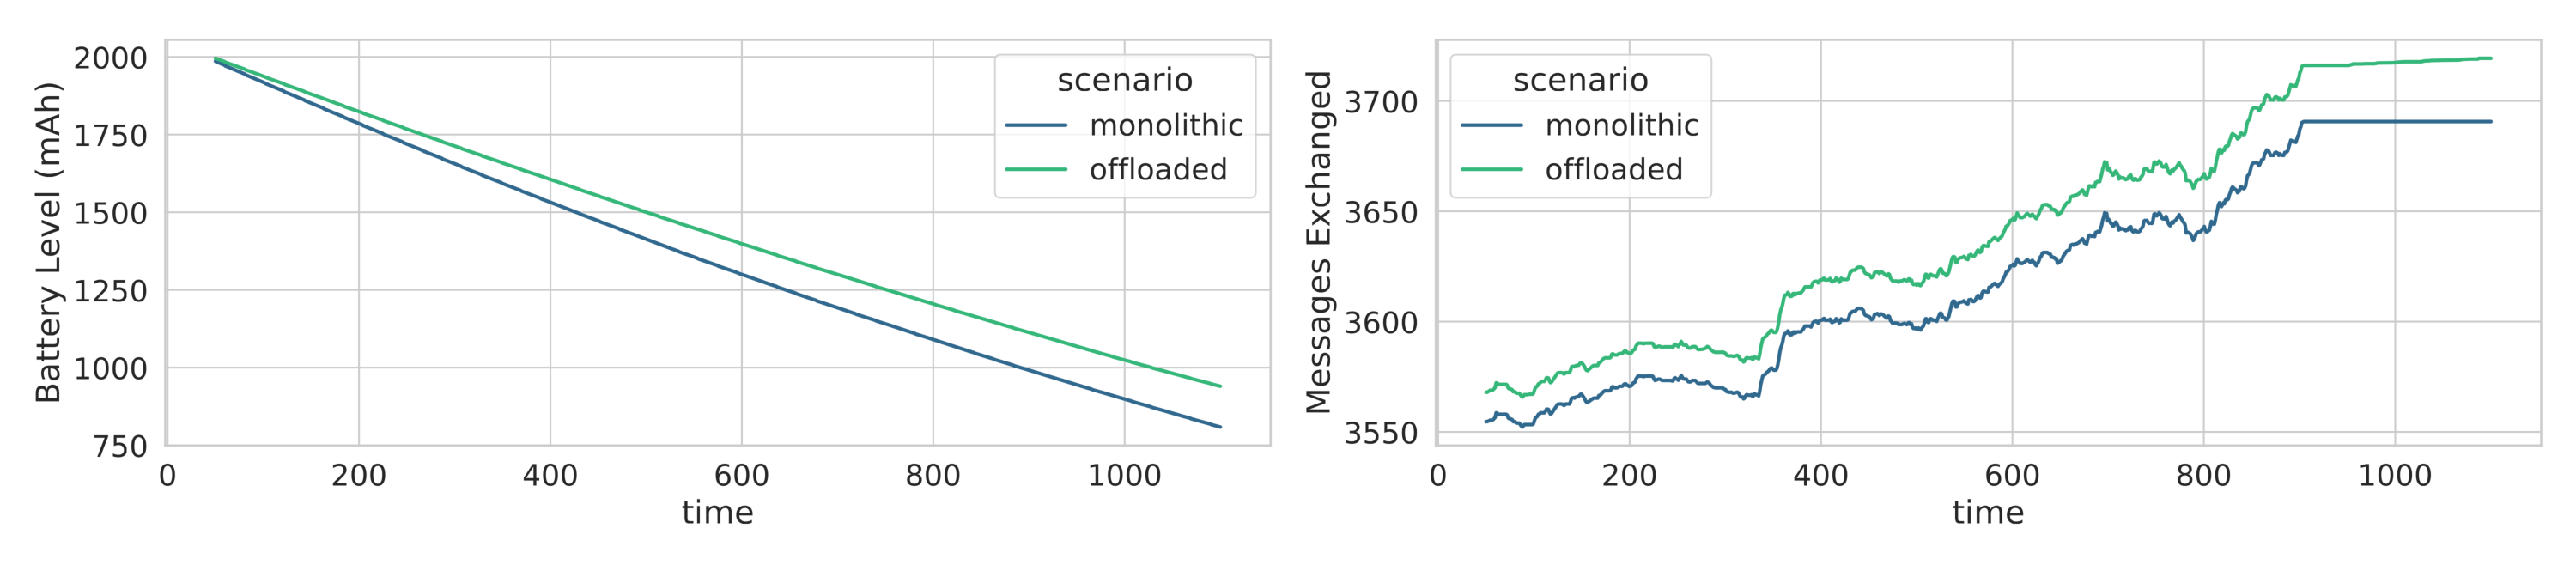
\includegraphics[width=\textwidth]{power-consumption.pdf}
    \caption[Battery level and message overhead under a monolithic and an offloaded deployment]{Average battery level (left) and cumulative messages exchanged (right) by application devices, under a monolithic and an offloaded deployment. Data from~\cite{DBLP:conf/acsos/FarabegoliVC24}.}
    \label{fig:power-consumption}
\end{figure}

The offloaded deployment leaves devices with more battery at the end of the run.
%
It exchanges slightly more messages in return, as the right-hand chart of \cref{fig:power-consumption} shows:
reaching Emergency Service at its surrogate and returning its result takes hops that a local execution does not need.
%
The cost is not paid in energy, since the offloaded devices are the ones with more battery left.
It is paid in bandwidth, in the extra messages the forwarding chain to the surrogate requires.

The rule obtains this result from the cheapest possible statement: one threshold, one component, and no coordination between devices.
%
It does not generalise beyond the signal and the component it was written for.
%
A second bottleneck, or a second component worth offloading under different conditions, would need a second threshold chosen by hand.

\section{A Field-based Reconfiguration Policy over Self-organising Coordination Regions}
\label{sec:global-self-organising-reconfiguration}

This section answers the same question as \cref{sec:battery-triggered-offloading}:
which infrastructural device should run the component an application device would rather not run locally.
%
The answer is no longer read off a single, locally observed number.

Every infrastructural device seeds a potential field weighted by its own current load.
%
A lightly loaded device's field reaches further into the network than a heavily loaded one's,
and each application device is claimed by the field that reaches it with the lowest potential~\cite{DBLP:journals/iot/FarabegoliPCV24}.
%
The construction is the self-organising coordination regions pattern already met in \cref{subsec:pulverization-validation}~\cite{DBLP:journals/fgcs/PianiniCVN21}, with one difference.
%
Leaders are not elected at a fixed grain: every infrastructural device is already a leader,
and its region-forming field encodes its own current load rather than distance alone.
A leader carrying more work therefore commands a smaller region.

A converge-cast brings each region's candidate components to its leader.
%
The leader accepts as many as its own capacity allows and casts the decision back over the same region,
so every application device either keeps its component locally or runs it on the infrastructural device that claimed it.
%
The regions resize themselves as load shifts, so the decision follows the whole network's topology instead of one local signal.
%
The policy still runs over the same infrastructure/application-device split the middleware maintains (\cref{chap:pulverization}).

The policy is evaluated against a local baseline that pins every application device to its nearest infrastructural device by hop count, whatever that device's load.
%
The networks hold a thousand hosts each, arranged as a scale-free and as a lobster, tree-like topology.
%
Two scenarios are simulated:
a variable load imposed externally on the infrastructural devices,
and a degradation and recovery in which batches of infrastructural devices are switched off and then progressively reactivated.
%
Quality of service is the share of application devices that manage to offload their component at all.

Across both scenarios and both topologies, the field-based policy reaches a higher quality of service than the local baseline once its regions have stabilised.
%
Stabilisation takes time, and quality of service can dip below the baseline's during that transient before recovering past it.
%
The policy also degrades and recovers more gracefully than the baseline when infrastructural devices fail.
%
Both advantages are larger in the scale-free topology than in the lobster one:
removing a node from a lobster network is far more likely to segment it,
cutting off the alternative routes the field-based policy needs to redirect load elsewhere~\cite{DBLP:journals/iot/FarabegoliPCV24}.

\section{A Declarative Planner for Green Deployments}
\label{sec:declarative-green-planning}

Declarative continuous reasoning was introduced above as Forti and Brogi's incremental repair of a stated deployment goal (\cref{subsec:declarative-deployment})~\cite{DBLP:journals/logcom/FortiBB22}.
%
The planner presented here follows the same idea, worked out over the deployment units defined in \cref{chap:pulverization}~\cite{DBLP:conf/coordination/BrogiCFFV25}.

Every deployment unit declares its hardware requirements and the maximum latency it tolerates towards the unit of the same macro-program it depends on most closely.
%
Every candidate host declares its available and total capacity, the power-usage effectiveness of running work on it, and the mix of energy sources that supplies it, with the associated carbon intensity.
%
A Prolog-based generator searches this space for an assignment of every deployment unit to a host that meets both kinds of requirement.
The requirements are stated as facts rather than computed by a bespoke solver, and the search is ordinary logic-program resolution.

The assignment problem is the same combinatorial one that is already too costly to solve exactly at scale (\cref{subsec:constraint-based-placement}).
%
The generator therefore tries candidate hosts from the least to the most carbon-intensive, reaching a low-carbon assignment quickly instead of exploring the space exhaustively.
%
For every candidate it considers, the same declarative program estimates the resulting energy draw and carbon emissions
from each host's load before and after the placement, its power-usage effectiveness, and the carbon intensity of its energy mix.

The generator is invoked at a fixed interval from inside Alchemist~\cite{DBLP:journals/jos/PianiniMV13}, the same simulator used to validate the model (\cref{subsec:pulverization-validation}).
%
Each time it runs, it receives the infrastructure's current state and returns a new assignment,
so the running deployment is periodically replaced by the one the search currently favours.
%
This is the repeated declarative repair of \cref{subsec:declarative-deployment}, driven here by an explicit energy and carbon objective rather than by an incremental reasoner reacting to a stated goal.

The published planner states its requirements over five deployment units per device: sensing, actuation, behaviour, state, and communication.
%
This is the fixed partitioning of a logical device that precedes the present model (\cref{sec:pulverization-motivation}).
%
The latency bound is stated towards the state unit, since the other four were designed to depend on it.

The search itself is not tied to that count or to a single hub.
%
A hardware requirement and a latency bound towards whatever a unit depends on are the kind of per-component declaration the bindings of \cref{subsec:macroprogram-dag} already make explicit for a macro-program of any size,
and the same Prolog predicates would run unchanged over a \ac{DAG} of arbitrarily many components.
%
What is evaluated below is the five-unit instantiation, not a macro-program pulverised into such a \ac{DAG}.
%
The mechanism generalises; the reported numbers do not speak on their own for deployments finer than five units per device.

The evaluation is synthetic.
%
A variable number of physical devices, each able to run every component locally, are placed uniformly at random in a two-dimensional area whose size grows with the device count.
%
Devices connect to one another within a range that also grows with the device count, a stand-in for a short-range radio, and all of them connect to a single cloud instance.
%
Each device's mix of energy sources follows a jittered sine wave, capped at 90\% green energy for devices and 50\% for the cloud.
%
The sine wave stands in for the day-night cycle in a grid's carbon intensity, the time-varying supply behind Wiesner et al.'s carbon-aware scheduling (\cref{subsec:energy-aware-orchestration})~\cite{DBLP:conf/middleware/WiesnerBSGT21}.
%
Each run simulates 720 simulated minutes of device movement, repeated ten times per configuration to average out random placement and mobility.
%
Two deployments are compared over the same runs.
The peer-to-peer baseline keeps every unit at its owner for the whole run, which is the monolithic deployment in this thesis's terms.
The other is recomputed by the generator every 30 simulated minutes.

\begin{figure}[t]
    \centering
    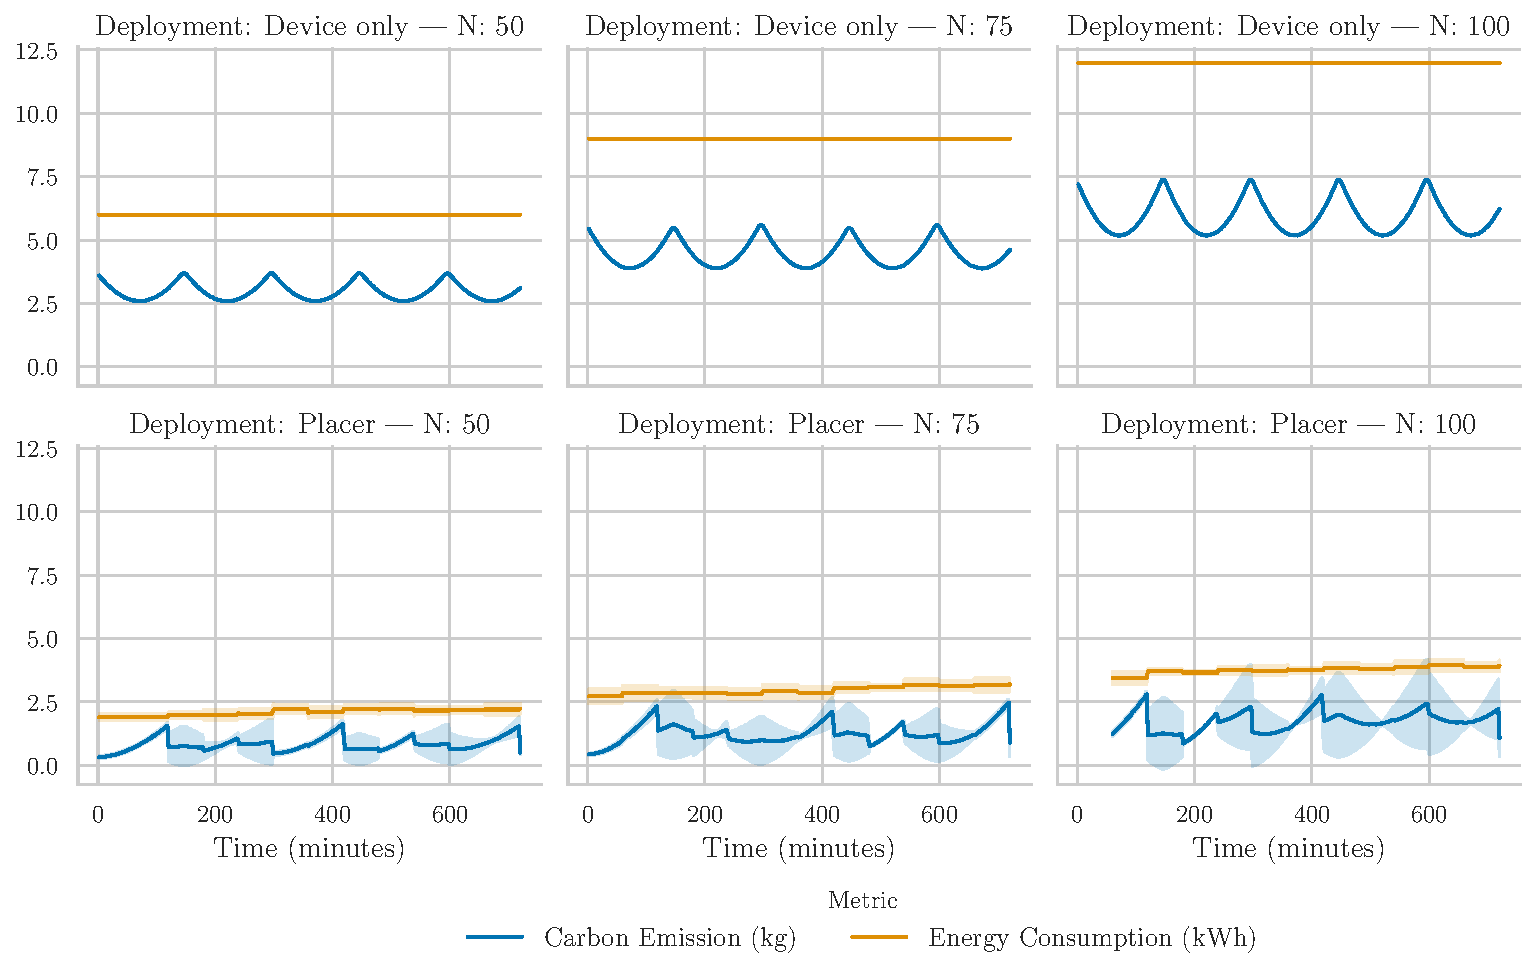
\includegraphics[width=\textwidth]{green-planner-carbon-energy.pdf}
    \caption[Energy consumption and carbon footprint under a peer-to-peer baseline and the declarative planner]{Overall energy consumption (orange) and carbon footprint (blue) across network sizes, comparing the peer-to-peer baseline (top row) with the deployment recomputed every 30 simulated minutes by the declarative planner (bottom row). Shaded bands show one standard deviation across ten repetitions. Data from~\cite{DBLP:conf/coordination/BrogiCFFV25}.}
    \label{fig:green-planner-carbon-energy}
\end{figure}

At every network size tested, the planner's deployment draws roughly a third of the energy the peer-to-peer baseline draws on the same network:
under 2 kWh for 50 devices, rising to 3.5 kWh for 100.
%
Its carbon footprint follows the same pattern (\cref{fig:green-planner-carbon-energy}).
%
The baseline's carbon footprint tracks the sinusoid of the energy mix exactly, because its deployment never changes and cannot exploit a momentarily greener mix elsewhere in the network.
%
The planner's footprint departs from that curve.
%
Recomputing the assignment every 30 minutes steers deployment units towards the host whose energy mix is least carbon-intensive at the time.
This is, for a pulverised deployment, the time-varying objective described for a single scheduled job in \cref{subsec:energy-aware-orchestration}.

\begin{figure}[t]
    \centering
    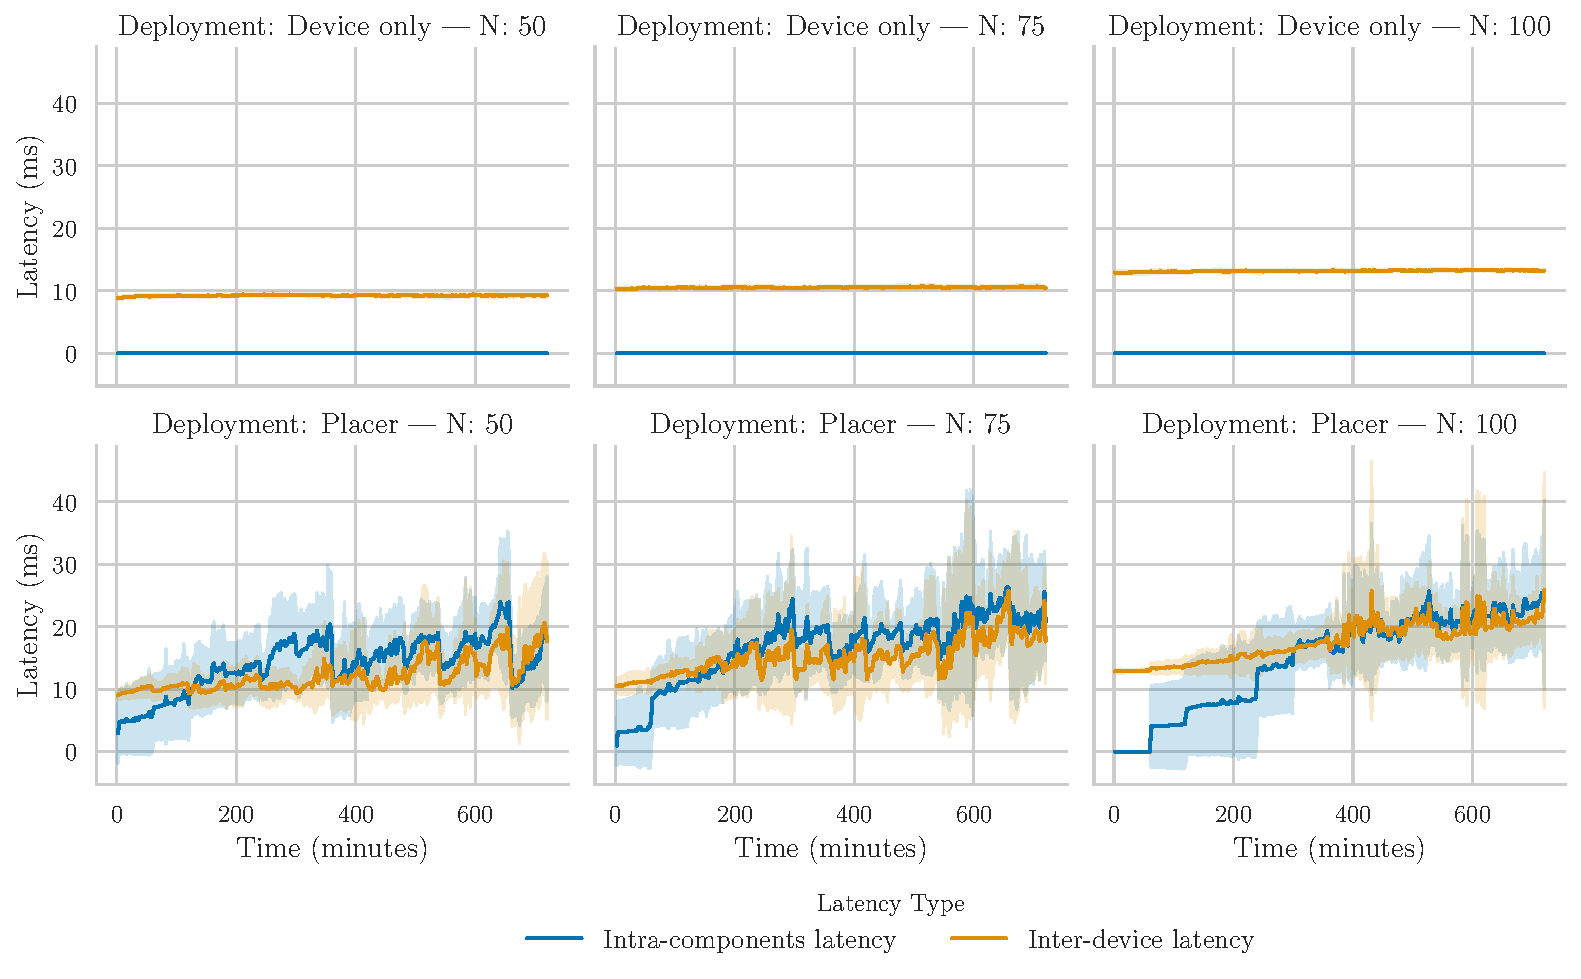
\includegraphics[width=\textwidth]{green-planner-latencies.pdf}
    \caption[Intra-component and inter-device latency under a peer-to-peer baseline and the declarative planner]{Intra-component latency (blue), the average delay a device experiences reaching its own deployment units wherever they have been placed, and inter-device latency (orange), the delay between the communication units of neighbouring devices, across network sizes, for the peer-to-peer baseline and the declarative planner. Shaded bands show one standard deviation across ten repetitions. Data from~\cite{DBLP:conf/coordination/BrogiCFFV25}.}
    \label{fig:green-planner-latencies}
\end{figure}

The energy reduction of \cref{fig:green-planner-carbon-energy} is not free.
\Cref{fig:green-planner-latencies} shows where it is spent.

Intra-component latency is the delay a device experiences reaching its own deployment units, now spread across more than one host.
%
It rises well above the near-zero, in-memory cost of the peer-to-peer baseline, which is the expected price of leaving units off the device that owns them.
%
The increase stays within the same order of magnitude as the network grows,
so the search keeps a device's units close together rather than scattering them further as the problem gets larger.

Inter-device latency is the delay between the communication units of neighbouring devices, and it is the one that matters for the collective computation itself.
%
It rises only slightly, even though nothing in the objective rewards keeping communicating units nearby.
%
Concentrating a device's units on a few nearby hosts keeps neighbouring devices' communication units close to one another as well.
%
The search itself scales:
computing a new assignment takes about 100 ms whatever the network size, well inside the 30-minute interval between replanning rounds~\cite{DBLP:conf/coordination/BrogiCFFV25}.

\section{Discussion}
\label{sec:deployment-reconfiguration-discussion}

All three evaluations show the same thing:
revising who runs a component at runtime reduces the quantity the policy targets, at a bounded secondary cost.
%
The offloading rule pays in messages, the planner in latency, and the field-based policy in a stabilisation transient.
%
None of them trades one non-functional gain for another outright.

None of them removes the work of deciding what counts as a good deployment either.
%
The offloading rule needs a person to fix a battery threshold and to choose, in advance, the one component worth offloading.
%
The field-based policy needs a person to decide that load is the quantity its regions compete over.
%
The planner needs a person to state the energy and carbon objective, the constraints the search must respect, and how often the search is repeated.
%
Every one of these policies is written by hand.

They differ in where that judgement is exercised and how far it reaches.
%
A single threshold says nothing about a second bottleneck, a second component, or a trade-off between two competing objectives.
Extending the rule means writing a new rule.
%
The field-based policy reasons over the whole network's topology and recovers from a failed host better than the other two.
That recovery depends on the topology it runs on, a dependence the threshold rule and the planner never face, since each was tested over a single topology.
%
The planner's objective covers several concerns at once: energy, carbon, and a latency bound enforced as a hard constraint.
Someone still had to write that objective and those constraints beforehand, and a further concern has to be stated by hand as well.

The next chapter drops that requirement (\cref{chap:heterogeneous-gnn}).
%
Instead of a rule or an objective fixed in advance,
a policy is trained to weigh the same non-functional concerns from experience,
under a condition none of the three policies of this chapter was built to see: network congestion.


\chapter{Learning-based Collective Task Offloading with Heterogeneous Graph Neural Networks}
\label{chap:heterogeneous-gnn}

% NOTE: background on RL, deep Q-learning, and GNNs lives in
% \cref{sec:ml-for-topologies}; reference back instead of re-explaining.


\chapter{A Demonstrator for Self-organizing Robot Teams}
\label{chap:demonstrator}

% NOTE: this chapter reports Project Emerge as the physical realisation of one
% deployment admitted by the model of \cref{chap:pulverization}. The pulverisation
% reading of its architecture is the thesis's own: the paper never uses that
% vocabulary. Aggregate computing background lives in
% \cref{subsec:aggregate-computing}; reference it instead of re-explaining.
% Two caveats must stay visible: the runtime exchanges neighbour messages in
% memory rather than over forwarding chains (\cref{sec:emerge-as-pulverisation}),
% and the chapter does not exercise
% \crefrange{chap:language-and-coordination}{chap:heterogeneous-gnn} --
% \cref{sec:emerge-discussion} states that gap rather than claiming otherwise.

Every claim this thesis has made about deployment has been checked in simulation:
the pulverisation model in Alchemist (\cref{subsec:pulverization-validation}),
the reconfiguration policies of \cref{chap:deployment-and-reconfiguration} in the same simulator,
and the learned offloading policy of \cref{chap:heterogeneous-gnn} against a simulated continuum.
%
Simulation is the right instrument for the questions those chapters ask, because it makes topologies, failures, and network sizes controllable.
%
It leaves one question open: whether a deployment the model admits can be built on real devices, with the sensing and actuation those devices have.

This chapter reports a system that answers it.
%
\emph{Project Emerge} is a toolchain that runs a single aggregate program on a team of physical mobile robots.
It was demonstrated publicly at the European Researchers' Night in 2024 and 2025.
%
Nine robots form spatial patterns and recover them after one of them is displaced by hand.
%
This chapter is concerned with where the computation runs.
The robots carry an ESP32 microcontroller and no aggregate runtime,
while a server evaluates the program on their behalf and returns actuation commands.
%
In the terms of \cref{chap:pulverization}, that arrangement is a deployment, with the robots as owners and the server as their shared surrogate.

That correspondence is the argument of this chapter. The paper does not make it.
%
Project Emerge was built to make aggregate computing demonstrable on hardware, and it describes its own architecture as centralised, without reference to pulverisation.
%
The deployment it arrived at, for reasons of its own -- microcontrollers too small to host a runtime -- is one of the deployments licensed by \cref{thm:deployment-independence},
and the freedom the theorem grants would let the same program run elsewhere unchanged.
%
The model left the deployment ``taken as given'' (\cref{sec:pulverization-discussion}); this chapter builds one such deployment on hardware.

The chapter follows the demonstrator from requirement to discussion:
what running a macro-program on real robots demands of the substrate (\cref{sec:emerge-requirements}),
the toolchain built to meet those demands (\cref{sec:emerge-architecture}),
how its deployment reads in the vocabulary of \cref{chap:pulverization} (\cref{sec:emerge-as-pulverisation}),
what the robots did (\cref{sec:emerge-demonstration}),
and what the demonstrator establishes and leaves untouched (\cref{sec:emerge-discussion}).
%
The contribution is published as~\cite{Farabegoli:2026:ProjectEmerge}, extending~\cite{DBLP:conf/coordination/AguzziBBCCDFPV25}.

\section{What a Physical Deployment Requires}
\label{sec:emerge-requirements}

Aggregate computing assumes a device that senses, computes, and actuates in rounds (\cref{subsubsec:ac-execution-model}).
%
A simulator supplies all three by construction.
On physical robots each has to be built, or substituted by something that stands in for it,
and a demonstrator's engineering effort goes into closing that gap.
%
Six requirements describe the gap.

\paragraph{Positioning.}
A macro-program that computes movement needs to know where its devices are.
%
Position alone is not enough:
a command to move in a direction is meaningless to a robot that does not know which way it is facing,
so the positioning system must report \emph{orientation} as well.
%
Outdoors this can be satellite positioning; indoors, where the demonstrator runs, it cannot.

\paragraph{Homogeneous program loading.}
One program specifies the behaviour of the whole team (\cref{sec:macro-programming}),
and every robot must be running it for the collective behaviour to be the one specified.
%
Loading it must not require shutting the team down.
%
During a switch from one version to another the two coexist,
and they must not interfere while they do, until every robot has moved across.

\paragraph{Neighbourhood policy.}
A device's neighbours are a dynamic set, and in a physical deployment membership is decided by physical facts:
proximity, line of sight, achievable data rate.
%
The substrate has to make that policy explicit and replaceable, rather than fixing one notion of adjacency.

\paragraph{Actuation agnosticism.}
The output of a round must not presuppose a chassis.
%
The program's output is an intention -- move this way, turn that way --
and translating an intention into wheel or rotor commands belongs to the platform, not to the program.
%
Without that separation the same program cannot run on two different robots.

\paragraph{Openness to platforms, and to where the program runs.}
The previous requirement concerns which robots a program can drive;
this one concerns which robots can drive themselves.
%
Platforms differ in computational capacity,
so the substrate must be able to evaluate the program on the robot, or remotely on a supporting host that does it on the robot's behalf.
%
This requirement matters most for this thesis,
and the demonstrator states it but satisfies only its remote half (\cref{sec:emerge-as-pulverisation}).

\paragraph{Interaction.}
Emergent behaviour is hard to trust when there is nothing to look at.
%
An operator needs to observe device states and the fields the program computes,
and to perturb the running system -- displace a device, change a parameter, swap the program -- while it runs.

\section{Architecture of the Demonstrator}
\label{sec:emerge-architecture}

Project Emerge meets those six requirements with five subsystems communicating over a single MQTT broker:
a localisation system, a neighbourhood manager, the aggregate runtime, a dashboard, and the robots themselves.
%
\Cref{fig:emerge-architecture} shows how they connect.
%
Because every exchange goes through one broker, a simulator can later replace the robots (\cref{sec:emerge-demonstration}):
nothing in the runtime knows whether the positions it reads come from a camera or from a simulation.

\begin{figure}[t]
    \centering
    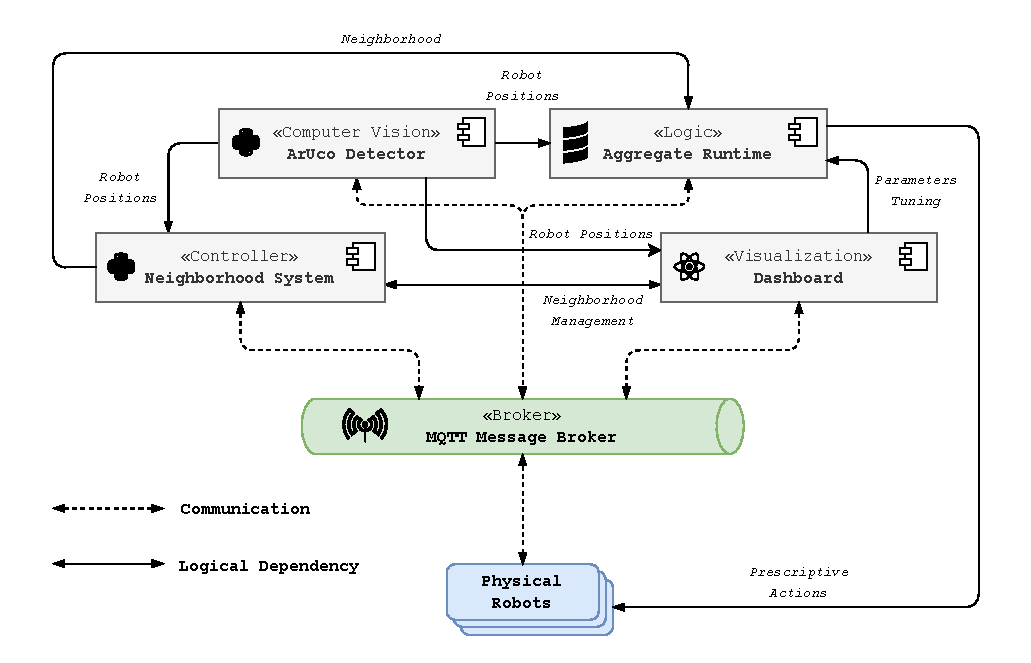
\includegraphics[width=0.85\textwidth]{emerge-architecture.pdf}
    \caption[System-level architecture of the demonstrator]{System-level architecture of the demonstrator. The localisation system tracks robot positions, the neighbourhood system maintains the adjacency relation, the aggregate runtime evaluates the collective program, and the dashboard supports monitoring and perturbation. Solid arrows are message flows through the broker; dashed arrows are logical dependencies. Adapted from~\cite{Farabegoli:2026:ProjectEmerge}.}
    \label{fig:emerge-architecture}
\end{figure}

Localisation is a camera above the arena and an ArUco marker on each robot,
processed by an OpenCV-based detector that publishes each robot's identifier, position, and orientation.
%
This discharges the positioning requirement without putting any sensor on the robot, a substitution examined in \cref{sec:emerge-as-pulverisation}.
%
The neighbourhood manager derives adjacency from those positions by spatial proximity,
and is kept separate from the localisation component so that a different policy can replace it.
%
The dashboard renders robots, their neighbourhood relation, and the current program,
and lets an operator drag a robot to a new position, retune a parameter, elect a leader, or load a different program.

\subsection{The Aggregate Runtime}
\label{subsec:emerge-runtime}

The runtime is written in Scala on ScaFi (\cref{subsec:cas-platforms}),
with the collective behaviours taken from MacroSwarm,
a library of field-based building blocks for swarm behaviour -- flocking, leader-based coordination, shape formation -- built on top of ScaFi~\cite{DBLP:conf/coordination/AguzziCV23}.
%
It is factored into four abstractions plus an entry point, and that factoring carries the requirements of \cref{sec:emerge-requirements} into code.\footnote{The toolchain, the companion rover hardware, and a reproducible capsule are released as open source: \url{https://github.com/Project-Emerge} and \url{https://doi.org/10.5281/zenodo.18224119}.}

An \texttt{Environment} models the physical context of one evaluation:
which robots are currently present, where each is, who its neighbours are, and what the sensors read.
%
An \texttt{EnvironmentProvider} builds that snapshot on demand,
its broker-based implementation assembling it from the localisation and neighbourhood messages received so far.
%
An \texttt{EnvironmentUpdater} performs the reverse translation, taking what a round computed and delivering it to the robots.
%
An \texttt{Orchestrator} evaluates the program:
given an environment, it computes, \emph{for each robot in it}, the program that robot is to run, evaluates it, and returns that robot's command.
%
The \texttt{AggregateService} composes the three into a loop that samples an environment, evaluates, and dispatches, at a fixed frequency.
%
\Cref{fig:emerge-execution-cycle} shows one turn of that loop.

\begin{figure}[t]
    \centering
    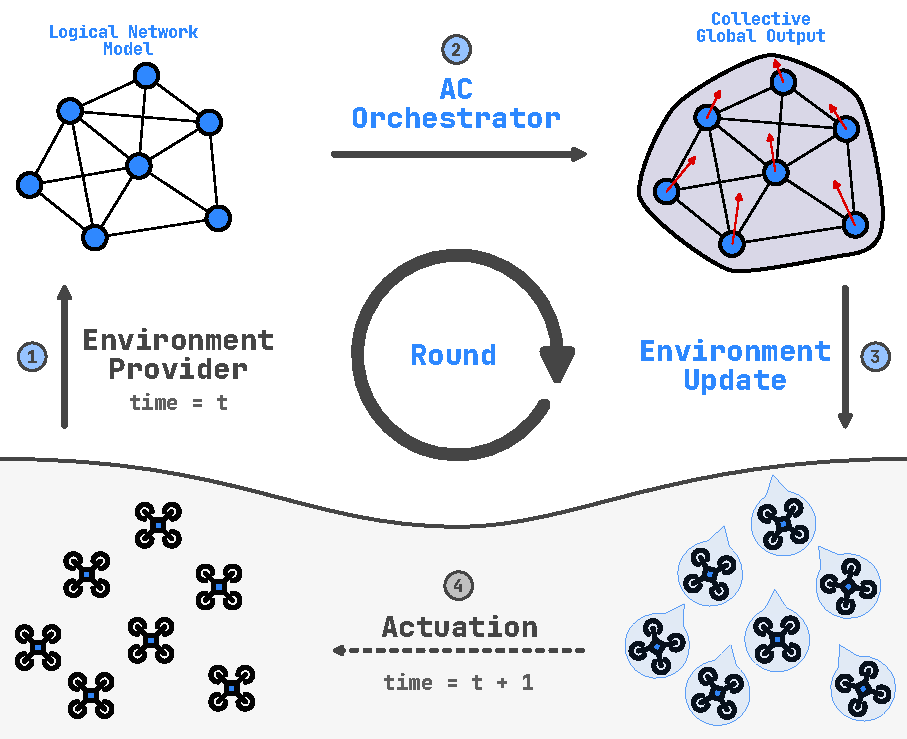
\includegraphics[width=0.6\textwidth]{emerge-execution-cycle.pdf}
    \caption[One evaluation cycle of the aggregate runtime]{One evaluation cycle of the aggregate runtime. The environment provider builds a logical network model from the physical robot states at time $t$; the orchestrator evaluates the aggregate program over it, producing actuation commands; the updater dispatches them; the robots execute them, carrying the system to $t+1$. Adapted from~\cite{Farabegoli:2026:ProjectEmerge}.}
    \label{fig:emerge-execution-cycle}
\end{figure}

Because the loop runs at a fixed frequency, it needs no explicit treatment of message ordering or timestamps:
each cycle consumes the latest message available on each topic and discards older ones.
%
A robot whose position update has not arrived is therefore evaluated against a stale pose rather than none.
%
This is a source of error the model already accounts for, since \cref{thm:deployment-independence} treats delayed and lost messages as transient perturbations that self-stabilising components absorb.

The boundary between program and platform is a small set of commands, shown in \cref{lst:emerge-actuation}:
rotate by a vector, move forward along a vector, hold, stop.
%
A MacroSwarm program yields one of these rather than a motor setting --
a prescriptive action, in the vocabulary of \cref{subsubsec:ac-execution-model}, that the robot is expected to attempt.

\noindent\begin{minipage}{\linewidth}
\begin{lstlisting}[
  style=scala3,
  caption={The boundary between an aggregate program and the robot platform. A program produces an intention; nothing in the type mentions wheels, rotors, or a chassis.},
  label={lst:emerge-actuation},
]
enum Actuation:
  case Rotation(towards: Vector2D)
  case Forward(along: Vector2D)
  case NoOp
  case Stop

trait BaseDemo extends AggregateProgram:
  override def main(): Actuation
\end{lstlisting}
\end{minipage}

The updater turns an intention into motion,
and in the current system it does so for differential drive:
a desired velocity vector becomes a pair of left and right wheel velocities.
%
Supporting a different chassis means writing a different updater; the program is unchanged.
%
The default program, \texttt{PointTheLeader}, shows the same boundary from the program's side:
it propagates a vector field outward from a leader elected through the dashboard,
using a gradient cast,
and returns a \texttt{Rotation} along that field so each robot turns to face the leader.

The runtime loads one program for the whole team, and can be told to switch to another over the broker while the team is running.
%
Because every subsystem speaks only to the broker,
a simulation engine can stand in for the robots and the camera together, publishing the same messages a physical arena would.

\section{The Deployment as a Pulverised One}
\label{sec:emerge-as-pulverisation}

The description just given is the demonstrator's own.
%
Restated in the terms of \cref{chap:pulverization}, it describes a deployment, subject to one qualification, stated below.
%
Nothing in this section is a claim the demonstrator makes about itself.

The nine robots are the application devices $\deviceIdSet$:
they carry the actuators the macro-program drives, and each of them owns an instance of its behaviour.
%
None of them executes that instance.
%
The server hosting the runtime is an infrastructural device, and it is the surrogate for every robot's behaviour component --
the case anticipated in \cref{subsec:forwarding-chains}, in which many owners forward the same component to one shared host.
%
The model permits it because component instances hold no state beyond their round-inputs,
which is why a surrogate can serve many owners as one without losing owner-specific behaviour.
%
The \texttt{Orchestrator} implements that collapse:
one process, one instance per robot, each evaluated against its own view of the network.
%
The broker relays messages without executing any, the role of the intermediate hop $\deviceId_1$ in \cref{fig:pulverization-forwarding}.
%
Writing the deployment predicate of \cref{subsec:forwarding-chains} for robot $\deviceId_j$ gives
%
\[
    \deploy(\deviceId_j,\ \component_{\mathit{beh}},\ \deviceId_j\ \mathit{broker}\ \mathit{server}),
\]
%
with actuation left at the owner.
%
Every pair of a device and a component is deployed and no chain repeats a device, so the deployment is correct in the model's sense.

One qualification limits what the restatement covers.
%
The broker carries the sensing and actuation traffic, but not the neighbour messages:
the runtime exchanges those in memory, inside the single process that hosts every instance, avoiding a network round trip per neighbour per round.
%
Under the model those messages would travel along forwarding chains.
%
The demonstrator therefore realises the limit case in which every chain terminates at the same host,
so the exchange the model would put on the network happens inside the surrogate instead.
%
The model admits that case -- it is the same collapsing of instances licensed in \cref{subsec:forwarding-chains} --
and the choice behind it is about performance, not about semantics.
%
A deployment that spread the same instances over several surrogates would have to send those messages, and would pay for them.

Sensing is the second place where the model's hypotheses constrain the design.
%
The robots' onboard sensors were not used:
they were replaced by the overhead camera, whose estimates of position and orientation reach the runtime through the environment provider.
%
The choice was made to keep a public demonstration reliable,
and in the model's terms it is a sensing component that does not run at its owner either.
%
A surrogate reads its own sensors, not the owner's,
so the substitution is sound only if what it samples is indistinguishable, as far as the component is concerned, from what the owner would have sampled --
the requirement that sensor state be uniform along the forwarding chain (\cref{subsec:deployment-independence}).
%
The requirement is met by construction:
the camera reports each robot's own position and orientation, the same quantities an onboard sensor would have reported for that robot.
%
The demonstrator thus satisfies the theorem's second hypothesis for the one sensing modality it uses,
and it satisfies the first by building its behaviours out of MacroSwarm's self-stabilising blocks (\cref{subsec:aggregate-computing}).

The arrangement the demonstrator settled on is not an alternative to the pulverisation model but an instance of it, arrived at independently,
and the reasons that forced it -- microcontrollers that cannot host a runtime, sensing better done from the ceiling than from the chassis --
are exactly the capability mismatches for which offloading is the answer given in \cref{subsec:forwarding-chains}.
%
The requirement of \cref{sec:emerge-requirements} that the program be executable \emph{either} on the robot \emph{or} on a supporting host
names the same freedom \cref{thm:deployment-independence} grants.
%
The demonstrator states that requirement and meets its remote half only.
%
Its own plan for the other half -- each robot running a local instance of the runtime, with localisation decentralised through radio ranging --
is, in the model's terms, the monolithic deployment in which every component runs at its owner.
%
The two are the extremes of one space; the mixed deployments lie between them,
and revising the choice among them at run time is the problem addressed in \crefrange{chap:deployment-and-reconfiguration}{chap:heterogeneous-gnn}.
The demonstrator does not yet do so.

\section{Demonstration and Observed Behaviour}
\label{sec:emerge-demonstration}

The demonstrator ran twice as a public exhibit, at the European Researchers' Night in 2024 and 2025,
in an indoor venue with an untrained audience walking through it.
%
The team was nine mobile robots on chassis designed and printed in-house,
each carrying an ESP32 microcontroller responsible for communication and low-level actuation, and a marker for the camera to track.

Five programs were demonstrated, chosen to exercise different coordination requirements:
a circle, in which the robots distribute along a circumference around a leader elected at run time;
a square, in which they converge on four corners while keeping the edges aligned;
a V-shape, two symmetric branches from a leader;
point-the-leader, in which each robot orients towards a designated one;
and line formations, horizontal and vertical, with uniform spacing along an axis.
%
Between them they cover symmetry, alignment, leader-based coordination, and global geometric constraints.
%
\Cref{fig:emerge-formations} shows four of them as they appeared in the venue.

\begin{figure}[tbp]
    \centering
    \begin{subfigure}{0.47\textwidth}
        \centering
        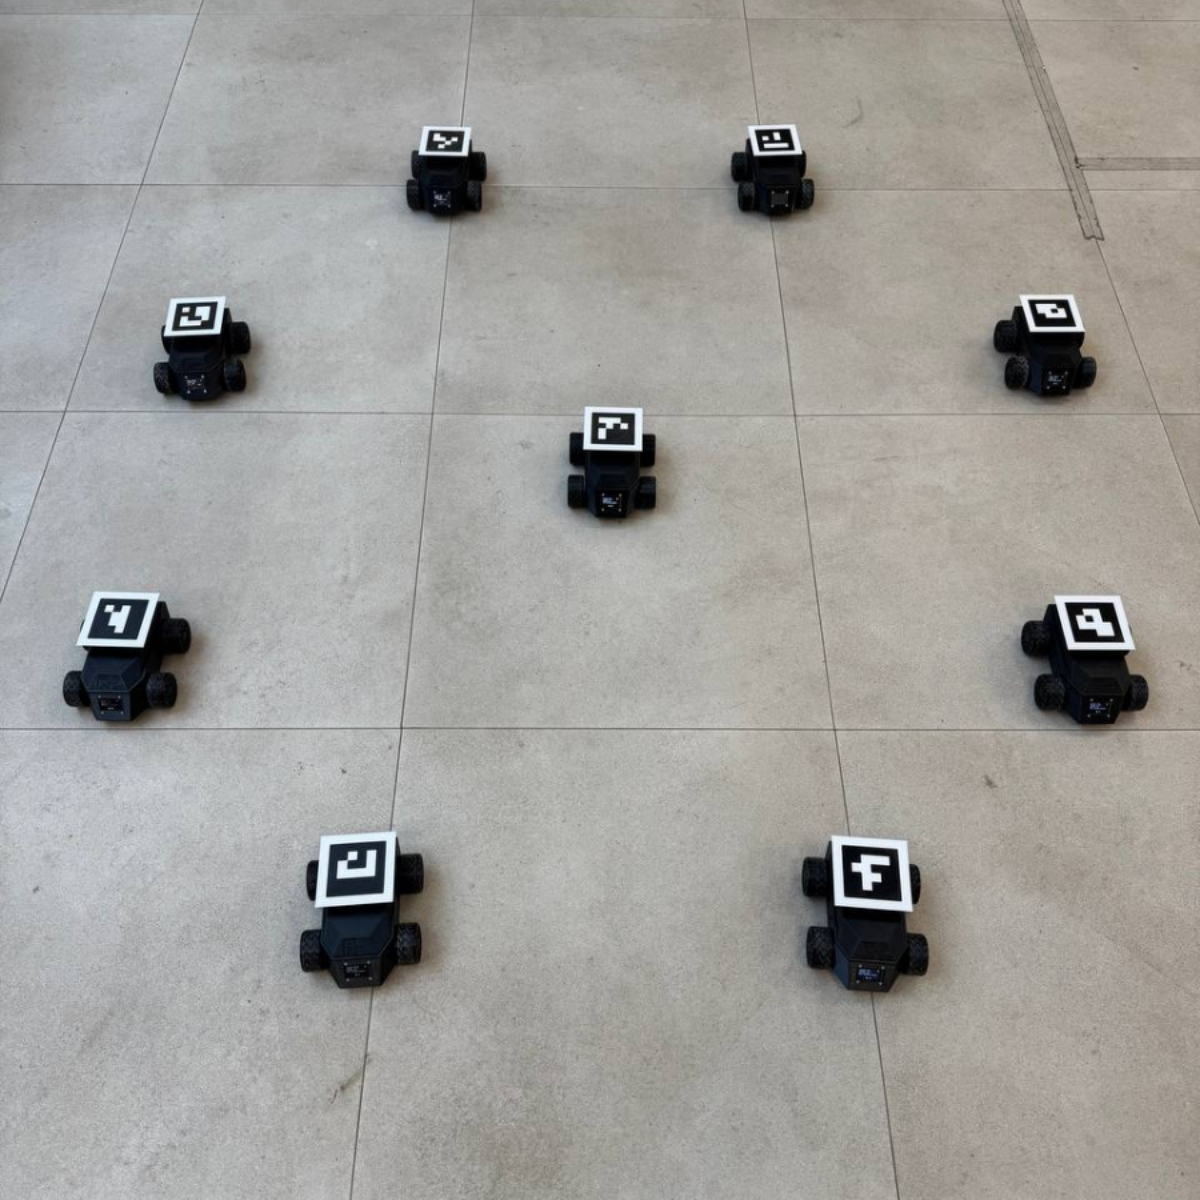
\includegraphics[width=\textwidth]{emerge-formation-circle.jpg}
        \caption{Circle}
    \end{subfigure}
    \hfill
    \begin{subfigure}{0.47\textwidth}
        \centering
        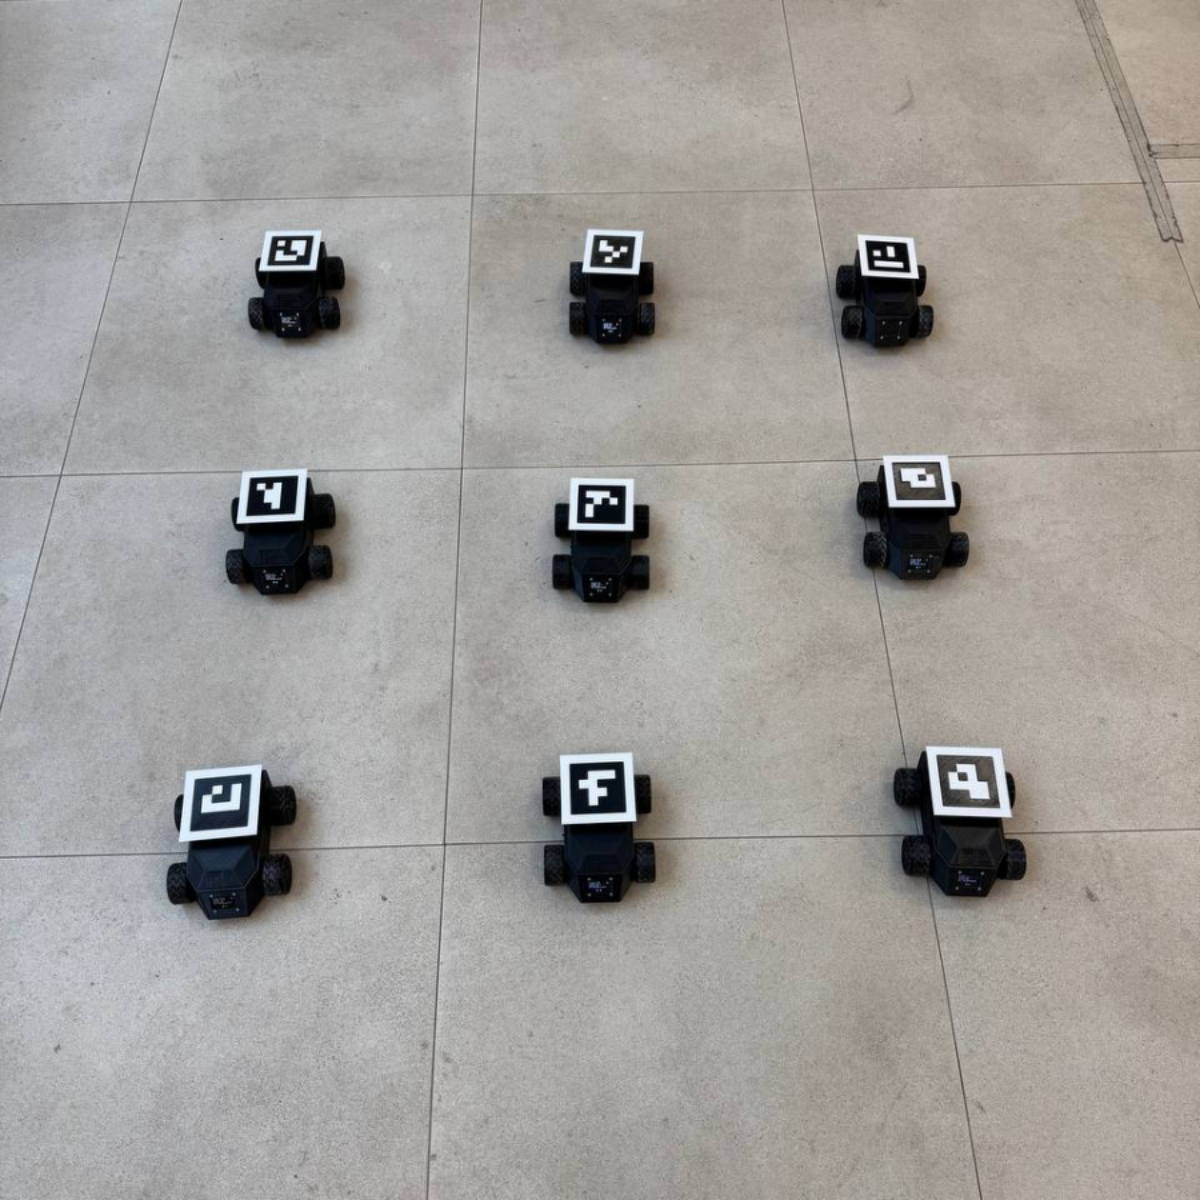
\includegraphics[width=\textwidth]{emerge-formation-square.jpg}
        \caption{Square}
    \end{subfigure}

    \vspace{0.6em}

    \begin{subfigure}{0.47\textwidth}
        \centering
        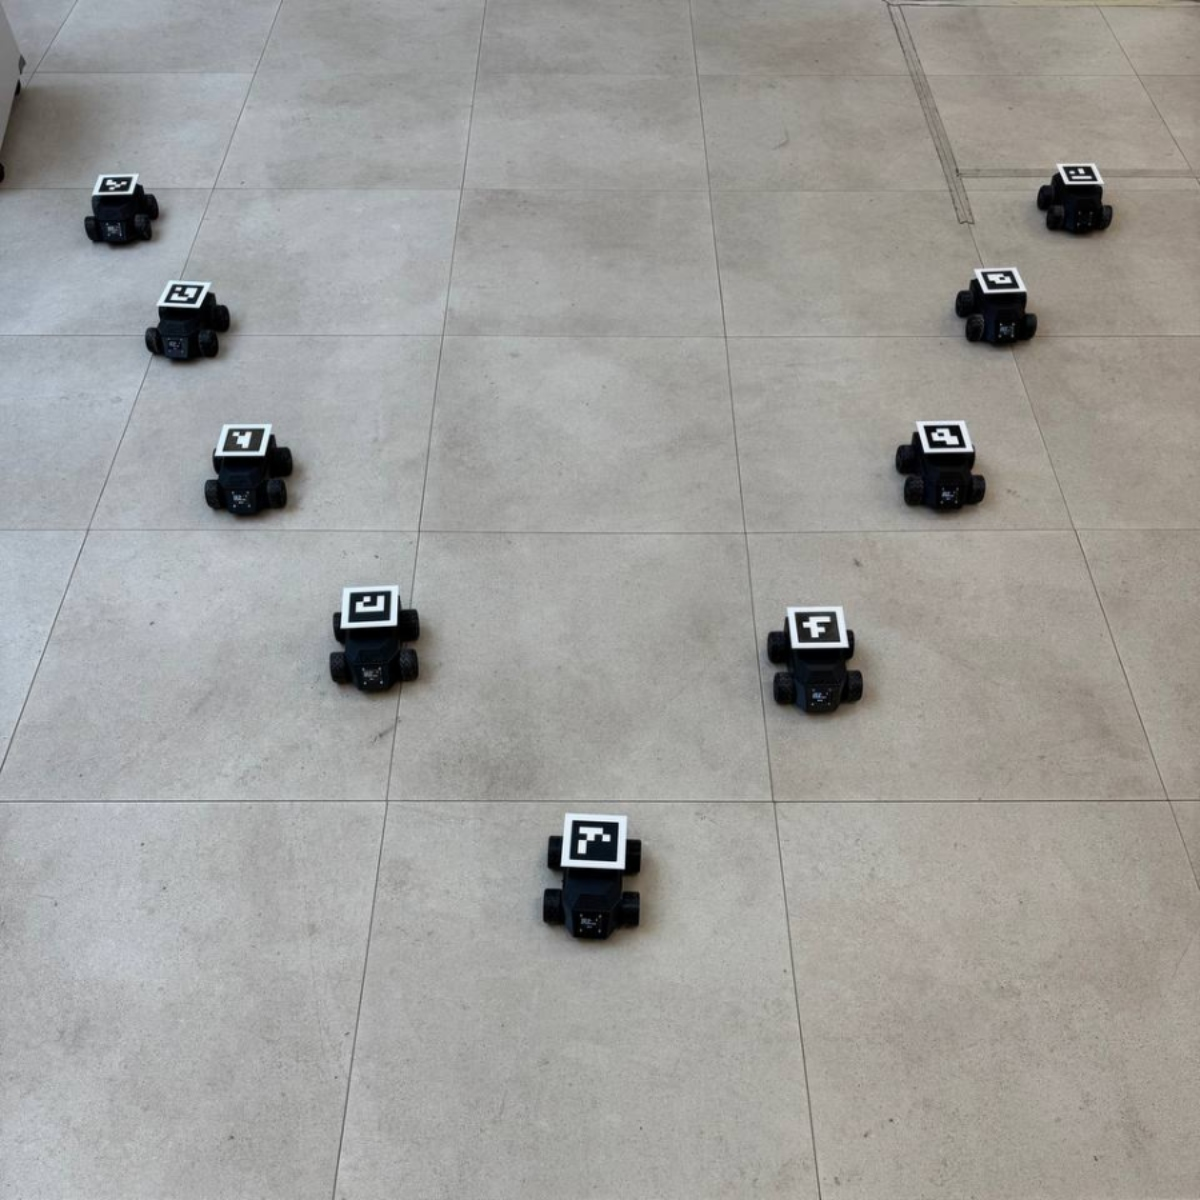
\includegraphics[width=\textwidth]{emerge-formation-vshape.jpg}
        \caption{V-shape}
    \end{subfigure}
    \hfill
    \begin{subfigure}{0.47\textwidth}
        \centering
        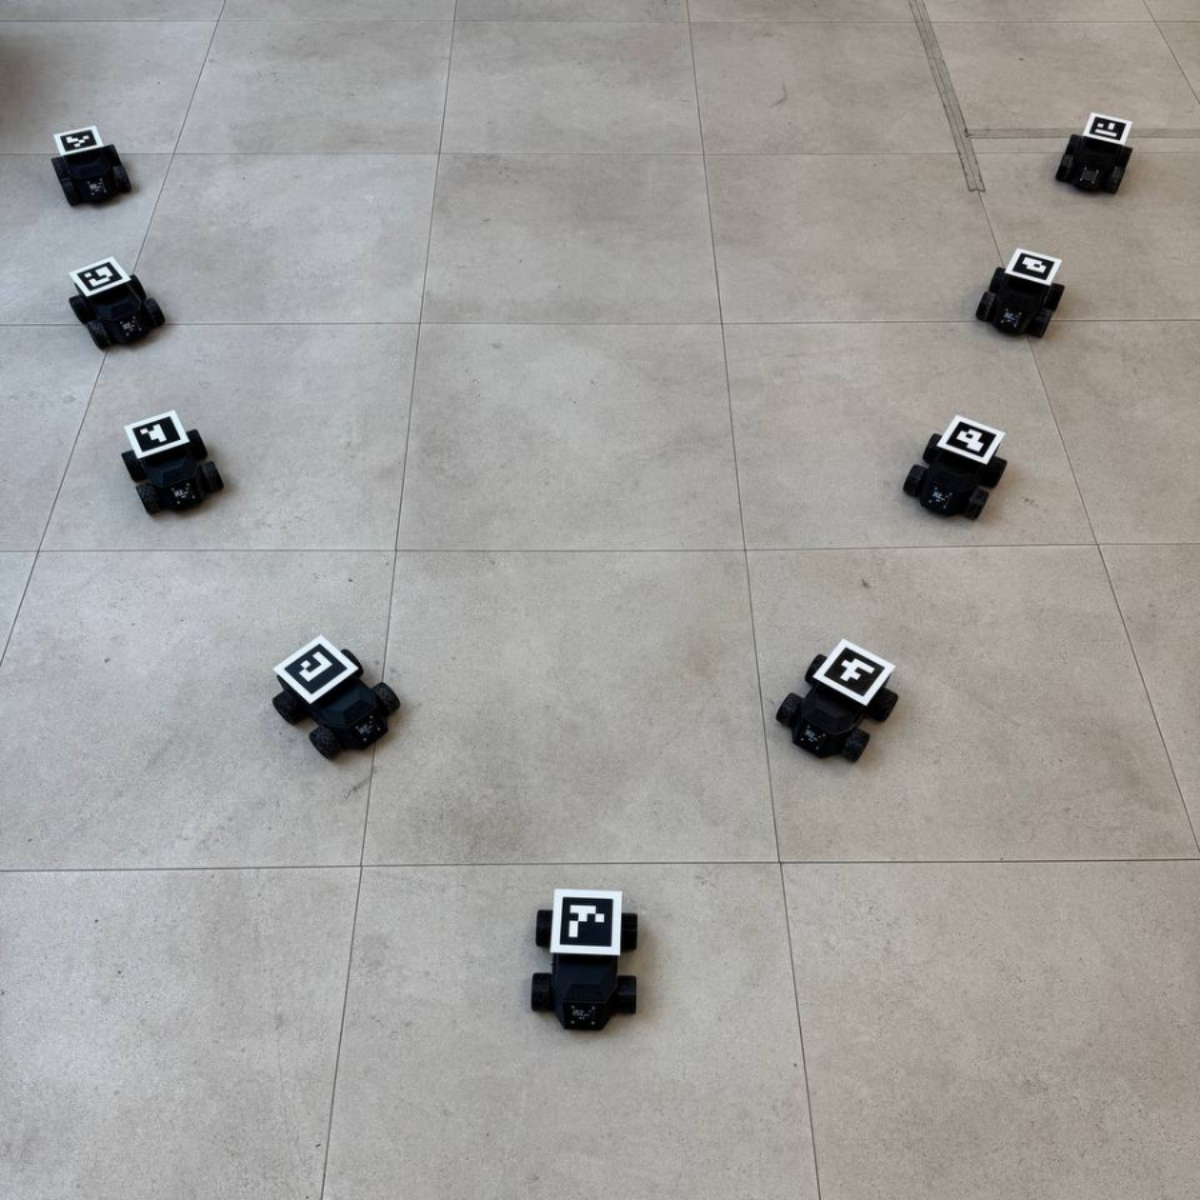
\includegraphics[width=\textwidth]{emerge-formation-pointleader.jpg}
        \caption{Point-the-leader}
    \end{subfigure}
    \caption[Spatial patterns formed by the robot team]{Four of the spatial patterns the team formed during the demonstration, each produced by a different aggregate program loaded into the running system. From~\cite{Farabegoli:2026:ProjectEmerge}.}
    \label{fig:emerge-formations}
\end{figure}

Programs were switched while the team was running, as the requirement of \cref{sec:emerge-requirements} demands.
The audience saw one formation dissolve into the next without the system being restarted.
%
The dashboard, shown in \cref{fig:emerge-dashboard}, was part of the exhibit rather than an operator tool,
since the neighbourhood relation it draws is otherwise invisible,
and a visitor could change the neighbourhood radius and watch the formation reorganise.

\begin{figure}[tbp]
    \centering
    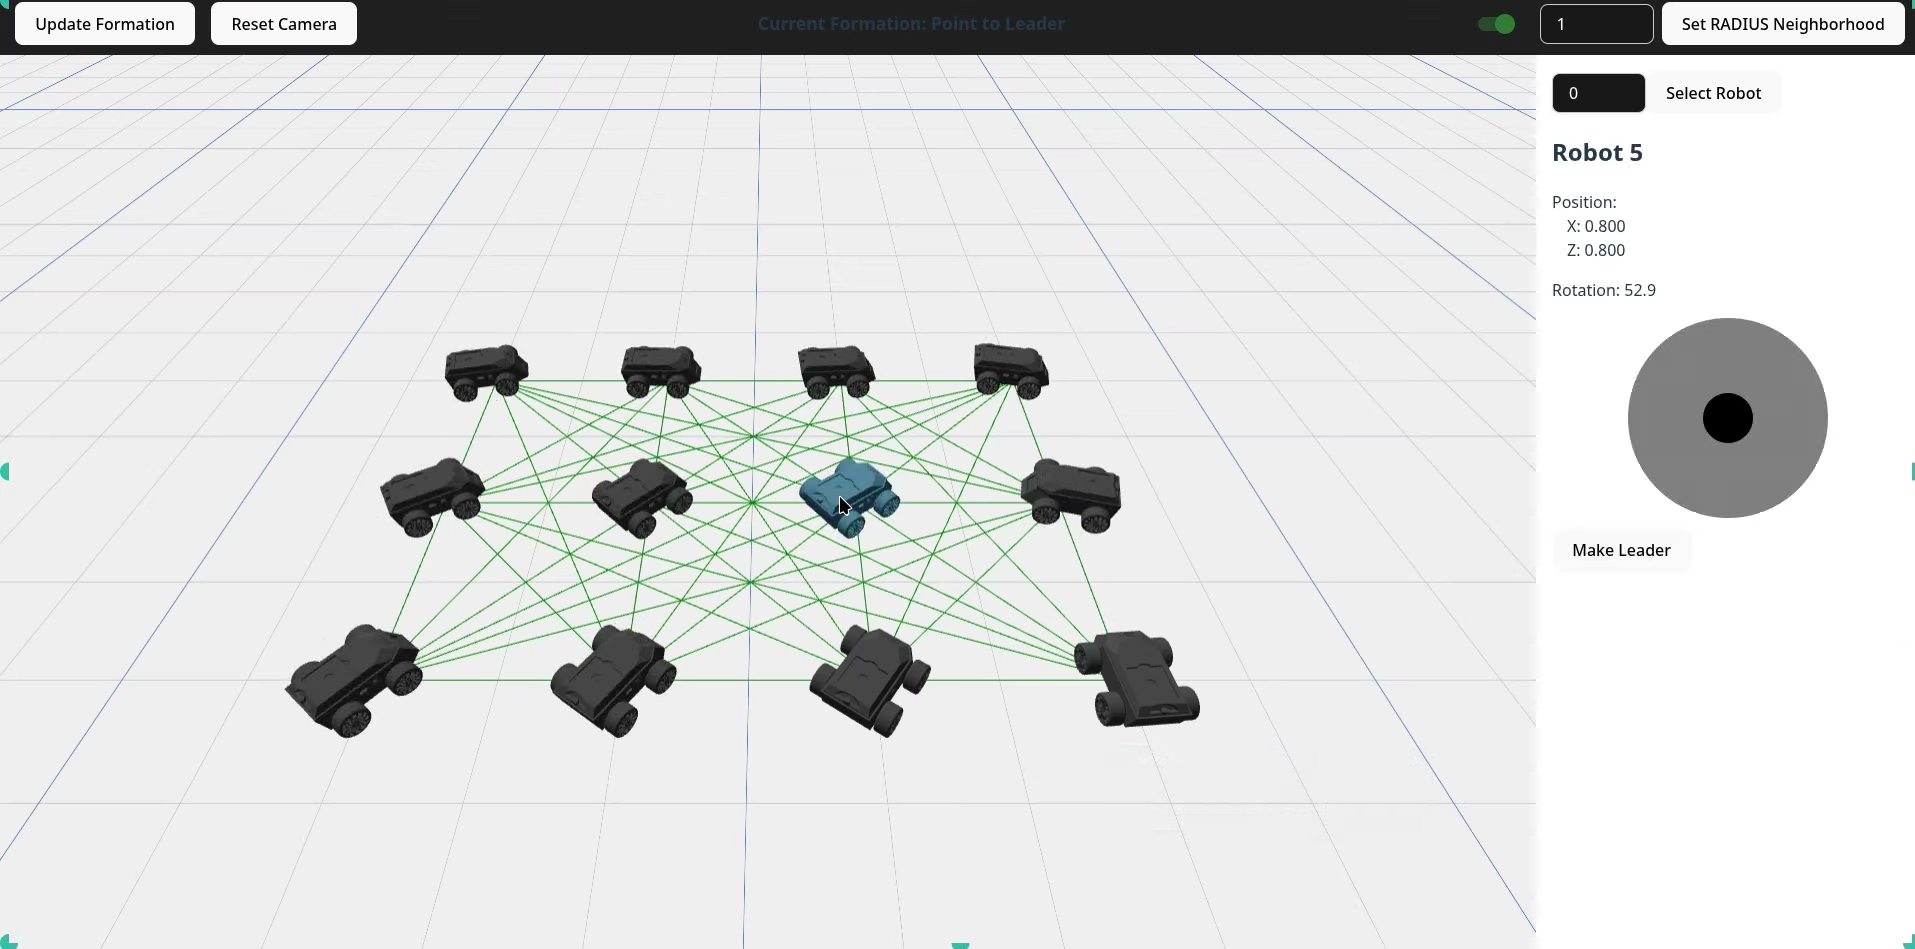
\includegraphics[width=\textwidth]{emerge-dashboard.png}
    \caption[The dashboard used to observe and perturb the running team]{The dashboard used to observe and perturb the running team. Lines between robots draw the current neighbourhood relation, which is otherwise invisible to an observer. The controls load a different aggregate program and retune the neighbourhood radius; selecting a robot exposes its state, a manual movement control, and the option to elect it leader. From~\cite{Farabegoli:2026:ProjectEmerge}.}
    \label{fig:emerge-dashboard}
\end{figure}

The property worth testing on hardware was self-stabilisation.
%
Simulation had already confirmed that an offloaded deployment converges where a monolithic one does (\cref{subsec:pulverization-validation}),
under the perturbations that study modelled: node mobility, and movement stopping partway through.
%
A physical arena admits perturbations neither of those covers, applied by hand and not scripted in advance.
%
Formations were disrupted in three ways:
displacing one or more robots mid-execution,
removing a robot from the arena and later putting it back,
and changing the formation parameters or the elected leader while the team was converging.
%
Removal and reinsertion is the most informative of the three, because it is node churn --
one of the perturbation classes the definition of self-stabilisation quantifies over (\cref{subsec:deployment-independence}) --
applied to hardware rather than to a simulated network.
%
In every case tried, the team absorbed the perturbation and recovered the formation without intervention.
%
\Cref{fig:emerge-selfhealing} shows one such recovery.

\begin{figure}[tbp]
    \centering
    \begin{subfigure}{0.32\textwidth}
        \centering
        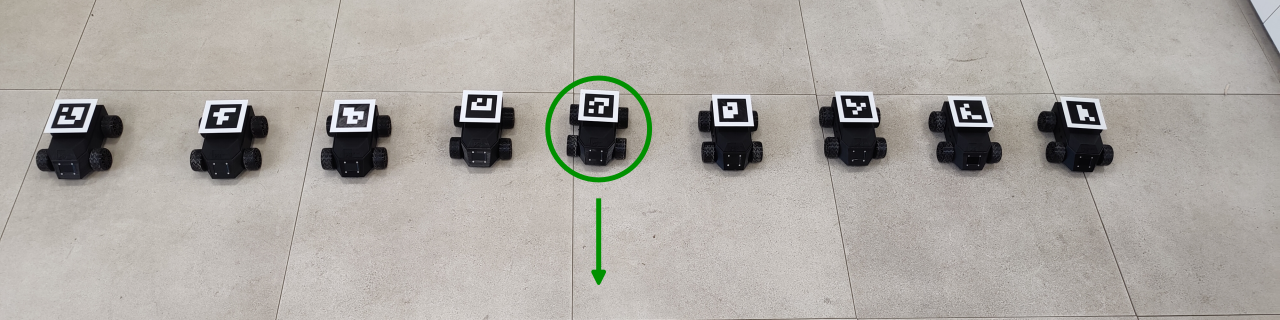
\includegraphics[width=\textwidth]{emerge-selfhealing-1.png}
        \caption{Formation reached}
    \end{subfigure}
    \hfill
    \begin{subfigure}{0.32\textwidth}
        \centering
        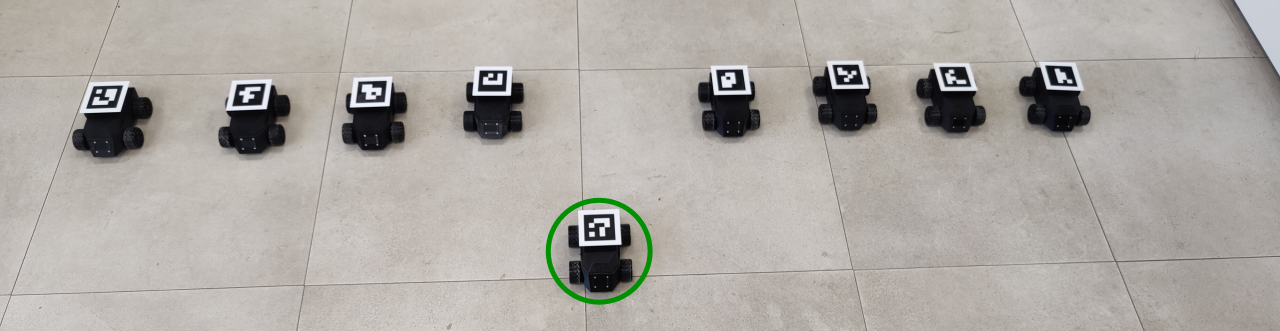
\includegraphics[width=\textwidth]{emerge-selfhealing-2.png}
        \caption{A robot displaced by hand}
    \end{subfigure}
    \hfill
    \begin{subfigure}{0.32\textwidth}
        \centering
        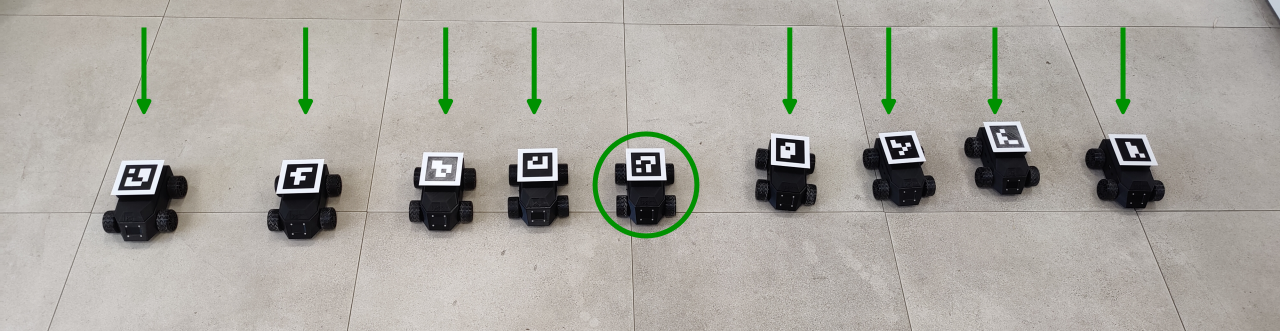
\includegraphics[width=\textwidth]{emerge-selfhealing-3.png}
        \caption{Formation recovered}
    \end{subfigure}
    \caption[Recovery of a line formation after manual perturbation]{Recovery of a line formation after a robot is displaced by hand during execution. From~\cite{Farabegoli:2026:ProjectEmerge}.}
    \label{fig:emerge-selfhealing}
\end{figure}

The evidence is qualitative.
%
The demonstration measured nothing.
It supports the claim that self-stabilisation survives physical embodiment and manual perturbation,
and no claim about how quickly, or about how recovery time compares across deployments.
%
A quantitative version of this experiment is within reach through the simulation engine that replaces the robots and the camera:
it exposes the same broker interface,
so a program validated against it and a program run in the arena are the same program under two sensing substrates.

\section{Discussion}
\label{sec:emerge-discussion}

The demonstrator establishes something narrow.
%
A deployment admitted by the model of \cref{chap:pulverization} has been built on real hardware and run in front of an audience.
%
That is evidence that the model's admissible deployments are not only simulable but realisable,
and that the capability mismatches motivating offloading in \cref{subsec:forwarding-chains} are the ones physical robots present.
%
The sensing substitution shows this most clearly:
condition \emph{(ii)} of \cref{thm:deployment-independence} reads as a technical hypothesis on paper,
and here it is a design decision -- put the sensor on the ceiling instead of the chassis -- that happens to satisfy it.

The demonstrator leaves much of the thesis untested.
%
Its deployment is fixed by hand before the system starts and never revised while it runs,
so it exercises none of \crefrange{chap:deployment-and-reconfiguration}{chap:heterogeneous-gnn}:
there is no reconfiguration policy, no declarative plan, and no learned offloading decision in it.
%
Its behaviour is one aggregate program rather than a macro-program decomposed into a \ac{DAG} of components,
so the finer-grained partitioning of \cref{subsec:macroprogram-dag} is not put to work either;
what is offloaded is the whole behaviour, as in the original five-role pulverisation.
%
It is written in ScaFi and MacroSwarm directly,
not through the unified capabilities of \cref{chap:language-and-coordination} nor with the generation support of \cref{chap:language-based-macroprogramming}.
%
And it reports no measurements.
%
The demonstrator is therefore a realisation of one point of the deployment space this thesis defines, on physical devices,
rather than end-to-end validation of the thesis as a whole.

Those gaps also make it the right place to exercise the rest.
%
The requirement it states and half-satisfies -- run the program on the robot or on a supporting host --
is a deployment choice, and its architecture already isolates that choice behind the environment provider and the updater.
The platform this thesis proposes would let a policy make that choice instead of an engineer.
%
Four steps would close the distance, each one connected to an earlier chapter.
%
Giving every robot a local runtime instance, with localisation decentralised through radio ranging, reaches the monolithic end of the deployment space,
at which point a policy has two endpoints to choose between rather than one.
%
Injecting communication delays into the simulation engine gives the mixed deployments between those endpoints a cost,
which is the precondition for a policy of \cref{chap:deployment-and-reconfiguration} or \cref{chap:heterogeneous-gnn} to have anything to optimise.
%
Repeating the perturbation experiments under controlled conditions, rather than by hand in a crowded room, turns this chapter's qualitative observation into a measured convergence time.
%
And generating the collective behaviours from a natural-language specification, as done for ScaFi in \cref{chap:language-based-macroprogramming},
would put the whole chain from specification to physical actuation under test at once.
%
The four are taken up again in \cref{chap:conclusions}.


% Detach the conclusions from Part III: top-level PDF bookmark, without
% introducing a dedicated \part (the ToC gap is added inside the chapter file,
% where the write order relative to the chapter entry is guaranteed).
\bookmarksetup{startatroot}
% Part-sized gap in the ToC, so the chapter does not read as part of Part III.
\addtocontents{toc}{\protect\addvspace{2.25em}}
\chapter{Conclusions}
\label{chap:conclusions}

% TODO(canovaccio): expand into full prose.
\lipsum[1]

\section{Answers to the Research Questions}
\label{sec:rq-answers}

% One subsection per question, each in the same four moves: (1) the question in
% one sentence; (2) the answer as a claim -- a declarative sentence that could
% be false, not a summary of what the chapter did; (3) the specific result
% backing it, named; (4) the boundary of the claim. "Yes, under hypotheses (i)
% and (ii) of \cref{thm:deployment-independence}" is an answer; "the thesis
% explored how pulverisation enables flexible deployment" is not one.
%
% RQ1 -> Chapter 5: \cref{thm:deployment-independence}, confirmed in simulation
% by \cref{subsec:pulverization-validation}. \Cref{chap:demonstrator} adds
% scoped realisability evidence -- one admissible deployment, built on physical
% robots -- and nothing more than that. It is not end-to-end validation:
% \cref{sec:emerge-discussion} states that it exercises none of
% \crefrange{chap:deployment-and-reconfiguration}{chap:heterogeneous-gnn}, uses
% neither \cref{chap:language-and-coordination} nor
% \cref{chap:language-based-macroprogramming}, and reports no measurements. Do
% not contradict that statement here.
%
% RQ2 -> Chapter 6: CaMiL's soundness result over the three paradigms, its 46
% use cases, and ScalaTropy's communication primitives -- with the price both
% designs pay, refusing programs the paradigms they unify would accept.
% RQ2.1 -> Chapter 7: the abstraction ladder decides the outcome, not model
% scale.
%
% RQ3 -> Chapters 8-9: three hand-written policies, each reducing the quantity
% it targets at a bounded secondary cost and each needing a person to state what
% a good deployment is, then a learned policy that removes that requirement,
% given a representation that keeps the continuum's heterogeneity and a
% collective summary.
\lipsum[1]

\section{Limitations}
\label{sec:limitations}

% Aggregate the limits the chapters already state, grouped by research question
% rather than restated chapter by chapter: three in
% \cref{sec:pulverization-discussion}, three in
% \cref{sec:llm-macroprogramming-discussion}, four in
% \cref{sec:idhgql-discussion}, and the gaps in \cref{sec:emerge-discussion}.
% Grouping them by question shows which answer is weakest -- RQ3, whose evidence
% is entirely simulated.
\lipsum[1]

\section{Future Work}
\label{sec:future-work}

% Four steps that would close the distance between the demonstrator and the rest
% of the thesis are named in \cref{sec:emerge-discussion}, which promises they
% are taken up here: a local runtime instance on every robot with localisation
% decentralised through radio ranging, communication delays injected into the
% simulation engine so the mixed deployments have a cost, the perturbation
% experiments repeated under controlled conditions, and the collective
% behaviours generated from a natural-language specification. That promise has
% to be kept. Also open, from \cref{sec:idhgql-discussion}: multi-objective
% methods that learn a set of policies covering the Pareto front instead of one
% policy per weight vector, distinguishing application devices by profile, and
% placing bound components jointly rather than independently.
\lipsum[1]


%----------------------------------------------------------------------------------------
% BIBLIOGRAPHY
%----------------------------------------------------------------------------------------

\backmatter

% \nocite{*} % comment this to only show the referenced entries from the .bib file
% TODO(canovaccio): remove \nocite{*} before the final version, so the
% bibliography only lists actually cited entries.
\bibliographystyle{alpha}
\bibliography{bibliography,background}

\end{document}